% !TEX root = ../main.tex

\chapter{基于生成式对抗网络的无监督式时间序列特征学习与应用}
\label{chap:gan}

\section{引言}

% 时间序列的重要性
一般的,时间序列数据由随时间变化的连续过程的采样点构成\cite{langkvist2014review},是生态、金融、医疗和工业等领域的重要数据资源\cite{esling2012time,gaber2005mining}。然而时间序列存在高维、高噪、时变等特点使其难以被开采利用,时间序列分析被认为是数据挖掘领域中最具挑战的十个问题之一,如何从时间序列数据中学习关键特征仍然是一个开放性难题\cite{langkvist2014review}同时也是机器学习和数据挖掘技术在PHM系统工程中得到有效应用的前提\cite{zhou2011latent, he2012integrated, patil2008failure, yan2004prognostic}。

近年来神经网络尤其是深度神经网络因其具有很强的特征学习能力受到了广泛关注并取得了许多突破进展\cite{lecun2015deep}。
即使对专业知识具有强依赖的领域,比如生物\cite{webb2018deep}、医疗\cite{mirowski2008comparing}和工业\cite{tsui2015prognostics}等领域也纷纷引入神经网络探寻突破。机器学习可分为监督式学习和无监督式学习,现有的优秀成果大多为监督式学习,需要大量的标记数据作为训练集\cite{radford2015unsupervised}。然而获取标记数据对于各领域任何时候都很困难。因此,无监督式学习逐渐成为焦点并在计算机视觉领域取得诸多进展\cite{lee2009convolutional,lecun2015deep,radford2015unsupervised}。随着深度学习在计算机视觉领域得到成功应用,越来越多的学者开始探索针对时间序列数据的无监督式学习解决方案\cite{langkvist2014review}。
%论文\inlinecite{langkvist2014review}注意到针对领域的特征设计面临昂贵和耗时的问题以及深度学习在的先进性,对可用的时间序列无监督式深度学习模型进行了较为全面的综述。
%主要包括限制性玻尔兹曼机、自动自编码机、循环神经网络、卷积神经网络和隐马尔可夫模型。

生成式模型对数据底层分布进行学习是实现无监督式学习的主要方法,目前最主流的生成式模型有全可视信念网络(FVBN)\cite{frey1998graphical}、变分自编码机(VAE)\cite{russakovsky2015imagenet}和生成式对抗网络(GAN)\cite{goodfellow2014generative}。GAN 因具有计算高效、抗过拟合、学习复杂分布、局限性少等优势倍受关注,并且大量实践表明GAN相较于其他主流生成式模型可以生成更高质量的样本。GAN的核心由两个神经网络构成,分别称为生成器和判别器。生成器负责学习数据的分布,判别器是一个二分类器负责准确辨识输入样本的真伪,两者相互博弈基于梯度下降和反向传播方法进行学习。这样的博弈一值持续直到判别器无法辨别样本真伪为止。此时的GAN,一方面,生成器已学习真实数据集分布并可生成逼真的样本;另一方面,判别器在通过不断训练之后已学习辨识数据的关键特征。目前已有大量研究分别从模型结构\cite{mirza2014conditional,denton2015deep,radford2015unsupervised}、模型理论\cite{chen2016infogan,arjovsky2017wasserstein}和模型应用\cite{isola2017image,ledig2016photo,reed2016generative,salimans2016improved}三个方面对GAN进行优化。
%在计算机视觉领域已有很多成果表明GAN可以学习有价值的特征、生成逼真的样本、可有效利用无标记数据实现无监督学习。

然而,GAN的应用目前仍局限于计算机视觉领域,鲜有针对时间序列数据的解决方案。论文\inlinecite{creswell2018generative}为信号处理领域对GAN的研究进展作了全面综述,但鲜有针对时间序列数据的成果。针对时间序列数据的研究,截至目前本文只关注到\inlinecite{esteban2017real}\inlinecite{yahi2017generative}\inlinecite{choi2017generating},然而他们提出的GAN都只针对医疗数据并且只在一个医疗时间序列数据集上进行验证,难以为普遍存在的时间序列提供支持。

% 时间序列分类方法大致可分为两种,即基于距离度量的分类方法和基于特征的分类方法,两类方法效果的优劣直接依赖特征的质量。
时间序列分类是时间序列挖掘的核心任务之一并且分类优劣直接依赖于特征的质量。基于传统机器学习的分类方法易受模型和数据影响,分类效果因模型和特征学习方法的不同存在较大差异,很难找到一个具有绝对优势的单一模型\cite{bagnall2017great}。由于神经网络的优秀表现,逐渐有学者采用深度学习方法解决时间序列分类问题并且较传统方法的优化效果显著\cite{cui2016multi,wang2017time}。其中基于卷积神经网络实现时间序列分类的论文\inlinecite{cui2016multi}证明时间序列其中一类关键特征——Shapelet,仅仅是卷积操作的一种特殊情况,再加上优秀的分类效果充分说明卷积操作对时间序列的处理能力。然而以上应用均基于监督式学习方法,在获取足够的标记时间序列数据仍面临巨大挑战时难以进行广泛应用。

% 明确本章的工作
综上所述,本文针对普遍存在的时间序列数据结合卷积神经网络和生成式对抗网络提出时间序列生成式对抗网络(TimeSeris Generative Adversarial Nets, TSGAN)。一方面,TSGAN 的生成器可以有效的学习时间序列数据集分布并生成逼真的多样化的时间序列,有效揭示数据底层特性。另一方面,将TSGAN的判别器作为特征转换器与K 近邻、支持向量机和逻辑斯蒂回归分类模型融合以形成半监督式时间序列分类框架,为时间序列分类任务以及其他机器学习任务提供新思路。
\section{背景知识}


\subsection{神经网络概述}

\begin{figure}[H]
\centering
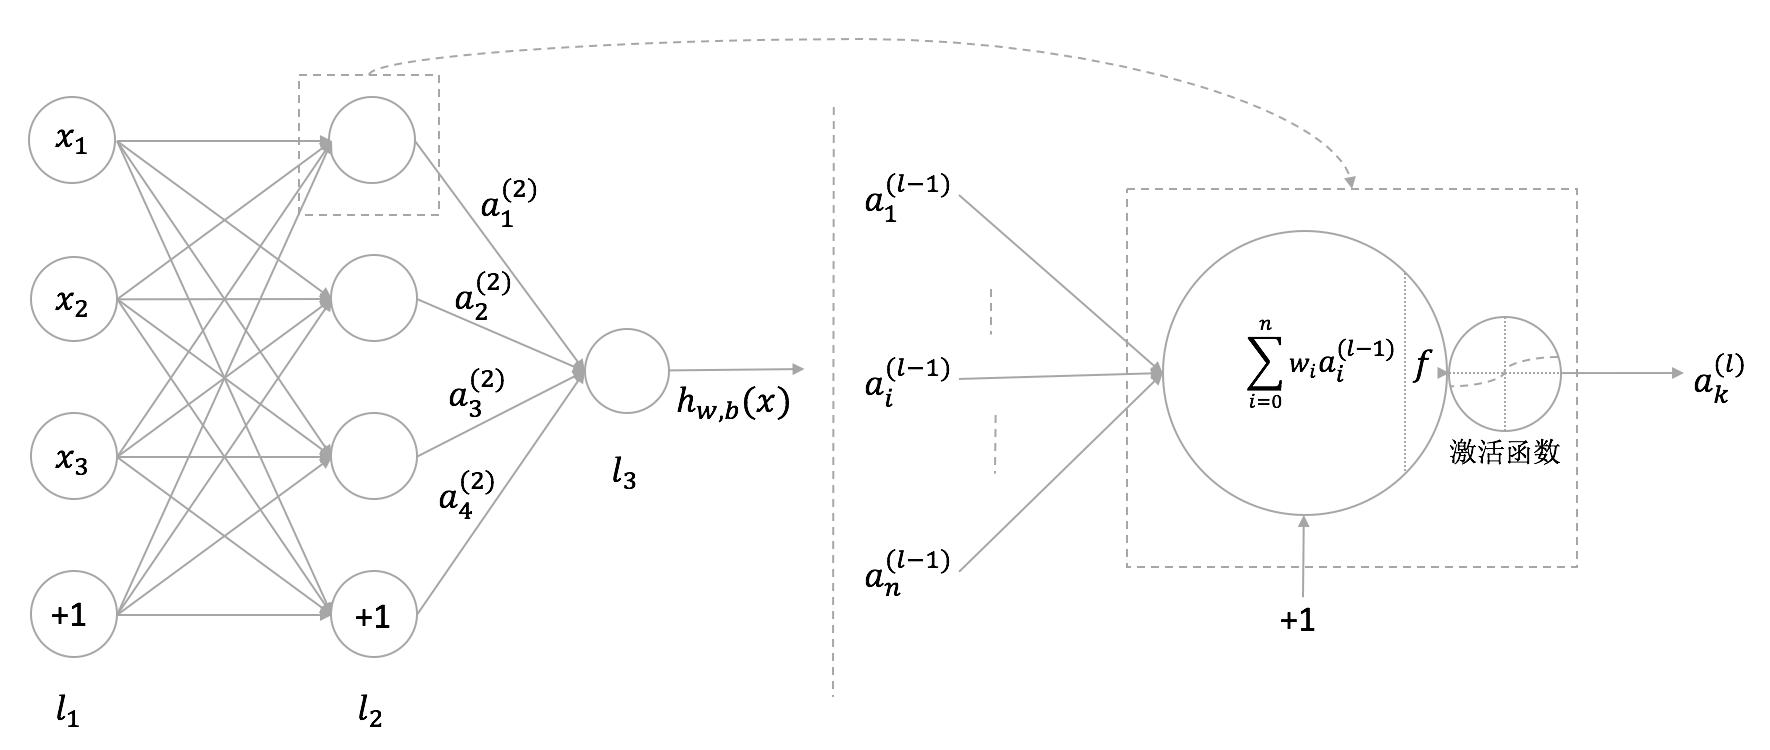
\includegraphics[scale=0.5]{figures/gan-neural-net.png}
\caption{(左)神经网络,(右)神经元}
\label{fig:gan-nn}
\end{figure}

(1)神经网络的基本结构

图\ref{fig:gan-nn}(左)是一个简单的三层神经网络,每一层都由若干个神经元构成。其中第一层为输入层,对应的神经元又称为输入神经元;第二层为隐藏层,对应的神经元称为隐藏神经元;第三层为输出层,对应的神经元称为输出神经元。每个神经元与其前一层所有神经元都有连接,因此这样的神经网络又称为全连接前馈神经网络。更复杂的神经网络无非是由更多隐藏层、更多神经元构成的复杂网络。

图\ref{fig:gan-nn}(右)是神经元结构,神经元负责接收并汇总来自前一层的信息由此作出是否激活的决策。设第$l$层第$k$个神经元的激活信号为$a_{k}^{l}$,其计算过程主要可分为以下两步:(1)汇总信息,假设前一层即第$l-1$层的$n$个神经元传来的信号为$<a_{1}^{l-1},...,a_{i}^{l-1}, ..., a_{n}^{l-1}>$;神经元通过求和得到汇总信息,即$\sum_{i=0}^{n}w_{i}a_{i}^{l-1}$,其中$a_{0}^{l-1}=1$表示神经元对应的偏置,对应图中的+1符号,这样的表示便于进行向量运算和矩阵运算。(2)基于汇总信息作是否激活的决策,即将汇总信息输入激活函数$f$,激活函数根据输入信号强度决定是否向网络下一层单元产生激活信号并计算激活信号强度,直观的激活函数可采用等式\ref{equ:gan-act-func-skip}的阶跃函数实现,只有当信号强度达到某一固定域值$\tau$时神经单元才被激活。综上,一个神经元的运算可归纳为等式\ref{eq:gan-neuron-calculation},依次类推可以计算第$l$层所有神经元的输出信号,以及神经网络中所有神经单元的输出信号。
\begin{equation}
\label{eq:gan-neuron-calculation}
a_{k}^{l}=f(\sum_{i=0}^{l-1}w_{i}a_{i})
\end{equation}

神经网络基于梯度下降算法进行训练,因此神经元的计算必须可导,那么上文介绍的直观阶跃函数\ref{equ:gan-act-func-skip}无法直接作为神经元的激活函数。激活函数可分为线性和非线性两种,由此可对应得到线性神经单元和非线性神经单元。线性激活函数定义为\ref{equ:gan-act-func-identity},一般用在回归问题的神经网络输出层。神经网络逐层叠加神经元其实相当于简单函数的嵌套叠加,如果其叠加的单元都为线性运算,那么最后得到的复杂表达式化简后还是线性运算,无法具有强大的抽象学习能力。因此神经网络中,尤其是负责特征学习的隐藏单元,基本都由非线性单元构成,嵌套叠加非线性函数形成的复杂函数具备对任何函数的近似能力,进而具有强大的抽象学习能力。其中神经元的非线性由非线性激活函数决定,并且激活函数需具有非线性、连续可倒性和单调性。以下是主流的激活函数:
% Sigmoid激活函数\ref{equ:gan-act-func-sigmoid},Tanh激活函数\ref{equ:gan-act-func-tanh},ReLU激活函数\ref{equ:gan-act-func-relu},PReLU激活函数\ref{equ:gan-act-func-parametric-relu}
\begin{itemize}
  \item Sigmoid 激活函数,又称 Logistic 函数,定义为\ref{equ:gan-act-func-sigmoid}。Sigmoid 最大的特点是其输出区间为[0,1],和概率的区间一致,因此可以天然的表达样本出现的可能性,通常用于针对二分类问题的神经网络最后一层,对于多分类问题通常使用Softmax函数。然而 Sigmoid 函数具有以下不足:(1)存在梯度消失问题,当神经网络逐渐加深时,梯度的强度将变得很微弱甚至可忽略不计,由此基于梯度的训练过程将停止;(2)输出区间没有以0为中心点,这将导致梯度更新因方向不同具有很大差距,并且这样的不对称性还会使优化过程更困难;(3)Sigmoid 对于很大或很小的输入会出梯度饱和现象;(4)Sigmoid 收敛速度慢。
  % 一般只用于输出层
  \item Tanh 激活函数,定义为\ref{equ:gan-act-func-tanh}。针对 Sigmoid 不以0为中心对称的问题,Tanh 对 Sigmoid 的输出进行变换,实际上$Tanh(x) = 2sigmoid(2x)-1$,由此可得到[-1,1]区间上的对称输出,使训练优化过程更容易。因为Tanh 激活函数是 Sigmoid 函数的变形,因此仍然存在梯度消失和梯度饱和的问题。
  % 一般只用于输出层
  \item ReLU 激活函数,定义为\ref{equ:gan-act-func-relu}。ReLU 解决了梯度消失问题,因此在深度学习中得到广泛应用,但值得注意的是ReLU只能用于神经网络的隐藏单元。ReLU收敛速度快,近期已有研究证明ReLU激活函数的收敛效率是Sigmoid和Tanh的6倍。ReLU的不足之处在于,当输入信号为负数时对应的函数值全为0,这可能会导致死神经元(Dead Neurons)问题,即有些神经元会在训练过程中停止更新。
  \item LeakyReLU、ParametricReLU和RandomizedReLU激活函数,解决解决了ReLU激活函中存在的死神经元问题。ParametricReLU 的定义为\ref{equ:gan-act-func-parametric-relu},特殊的当$\alpha = 0.01$时为LeakyReLU,训练时若通过随机算法在$\alpha$取值范围内随机确定参数,则称为RandomizedReLU。
\end{itemize}

对于激活函数的选择很难有确切的定论,目前 Sigmoid 和 Tanh 激活函数已很少用于神经网络的隐藏单元,通常根据问题的需要用于输出单元。当下的神经网络,尤其是卷积神经网络和深度神经网络的隐藏单元基本都选用ReLU函数和基于此的改进比如LeakyReLU,ParametricReLU和RandomizedReLU。
% 激活函数的 reference
% !!对激活函数的优缺点和发展介绍得比较清晰:https://towardsdatascience.com/activation-functions-and-its-types-which-is-better-a9a5310cc8f
% 简单概括,其中的表格和wiki的类似:https://towardsdatascience.com/activation-functions-neural-networks-1cbd9f8d91d6
% wiki,有一个很全的表格:https://en.wikipedia.org/wiki/Activation_function
% 最开始看到的,但废话还是比较多,不好:https://medium.com/the-theory-of-everything/understanding-activation-functions-in-neural-networks-9491262884e0
% tf activation function: tf.nn.relu, tf.nn.relu6, tf.nn.crelu, tf.nn.elu, tf.nn.selu, tf.nn.softplus, tf.nn.softsign, tf.nn.dropout, tf.nn.bias_add, tf.sigmoid,tf.tanh
\begin{subequations}
\begin{align}
a = f(x) &= Skip(x) = \left\{\begin{matrix}
1 & x \geqslant \tau  \\ 
0 &  x < \tau  
\end{matrix}\right. , a \in \{0, 1\} \label{equ:gan-act-func-skip} \\
a = f(x) &= Linear(x)=x , a \in (-\infty, \infty) \label{equ:gan-act-func-identity}\\
a = f(x) &= Sigmoid(x) = \frac{1}{1+e^{-x}} \label{equ:gan-act-func-sigmoid}, a \in [0, 1] \\
a = f(x) &= Tanh(x) = \frac{1}{1+e^{-2x}} - 1 \label{equ:gan-act-func-tanh} , a \in [-1, 1] \\
a = f(x) &= ReLU(x) = \left\{\begin{matrix}
x & x \geqslant 0 \\ 
0 &  x < 0
\end{matrix}\right. , a \in [0, \infty) \label{equ:gan-act-func-relu}\\
a = f(x) &= PReLU(x) = \left\{\begin{matrix}
x & x \geqslant 0 \\ 
\alpha x &  x < 0, abs(\alpha) \leq 1
\end{matrix}\right. , a \in (-\infty, \infty) \label{equ:gan-act-func-parametric-relu}
\end{align}
\end{subequations}

(2)神经网络的训练

设有$m$个样本的训练集,表示为$\{(x^{(1)}, y^{(1)}), ..., (x^{(i)}, y^{(i)}), ..., (x^{(m)}, y^{(m)})\}$。令$W_{i,j}^{l}$ 表示第\emph{l}层的第j个神经元到第$l+1$层的第\emph{i}个神经元的权重;$z_{i}^{l}$表示第\emph{l}层第\emph{i}个神经元的求和结果;$a_{i}^{l}$表示第\emph{l}层的第\emph{i} 个神经元的输出,具体的对于输入层$a_{i}^{1} = x_{i}$,对于隐藏层$a_{i}^{l}$为激活函数的计算结果,特殊的$a_{0}^{l}$表示偏置,对应权重为$W_{i,0}^{l}$。

设神经网络最后的输出为$h_{W}(x)$,易知$ h_{W}(x) = a^{l}$。由此可得单个样本输入$(x,y)$的损失函数定义为等式\ref{eq:gan-nn-cost-func},实际上是估计值和真实值之间的均方误差。对于整个数据集的损失函数为等式\ref{eq:gan-nn-loss-func},其中$n_{l}$表示神经网络的层数,$s_{l}$表示第\emph{l}层的神经元个数。等式\ref{eq:gan-nn-loss-func}由两部分组成,第一部分为所有样本的均方误差,第二部分为正则化项,定义采用的是$L_{2}$正则,$\lambda$为正则项的权重,值得注意的是偏置项不惩罚。
\begin{equation}
\label{eq:gan-nn-cost-func}
J(W;x,y) = \frac{1}{2}\left \| h_{W}(x) - y \right \|^{2}
\end{equation}
\begin{equation}
\label{eq:gan-nn-loss-func}
J(W) = [\frac{1}{m}\sum_{i=1}^{m}J(W;x^{(i)}, y^{(i)})] + \frac{\lambda}{2}\sum_{l=1}^{n_{l}-1}\sum_{i=1}^{s_{l}}\sum_{j=1}^{s_{l-1}}(W_{i,j}^{l})^{2}
\end{equation}

神经网络优化的目标是最小化损失函数,而梯度是函数上升最快的方向,那么梯度的反方向就是函数下降最快的方向,因此神经网络采用梯度下降的寻优方法获取最优解。其核心思想为,从某一初始值开始,每次都找到当前梯度最大的方向,然后沿这一方向的反方向对函数的各参数进行更新,即通过等式\ref{equ:gan-nn-update}对权重进行更新,其中$\alpha$为学习率。
\begin{equation}
\label{equ:gan-nn-update}
W_{i,j}^{l} = W_{i,j}^{l} - \alpha \frac{\partial J(W)}{\partial W_{i,j}^{l}} 
\end{equation}

神经网络的训练过程为对于每个输入样本(x,y)重复进行以下操作:
% 【梯度下降,随机梯度下降?区别是否要说?】
\begin{enumerate}[1.]
  \item 基于前向传播的方式计算神经网络每个神经元的输出,即依次对$2,3,..,n_{l}$层网络的各个神经元进行如下计算
  \begin{enumerate}
    \item $z_{i}^{l} = \sum_{j=0}^{n}W_{i,j}^{l-1}a_{j}^{l-1}, a_{0}^{l-1}=1$
    \item $a_{i}^{l} = f(z_{i}^{l})$
  \end{enumerate}
  \item 计算神经网络最后一层(第$n_{l}$层)的各个神经元对误差的反馈因子:

  $\delta_{i}^{n_{l}} = \frac{\partial \frac{1}{2} \left \| y - h_{W}(x) \right \|^{2}}{\partial z_{i}^{n_{l}}} = -(y_{i}-a_{i}^{n_{l}} )f'(z_{i}^{n_{l}})$

  \item 基于后向传播的方式计算神经网络每个神经元的误差反馈因子,即依次对$l$($l=n_{l}-1, n_{l}-2, ..., 2$)层的神经单元 进行以下计算:

  $\delta_{i}^{l} =(\sum_{j=1}^{s_{l+1}}W_{j,i}\delta_{j}^{l+1})f'(z_{i}^{l})$

  \item 同时对网络各个节点的权重进行更新:

  $W_{i,j}^{l} = W_{i,j}^{l}- \bigtriangledown W_{i,j}^{l}, \bigtriangledown W_{i,j}^{l} = \frac{\partial J(W;x,y)}{\partial W_{i,j}^{l}} = a_{j}^{l}\delta_{i}^{l+1}$

\end{enumerate}

\subsection{卷积神经网络概述}
% reference: 
% http://cs231n.github.io/convolutional-networks/
% https://ujjwalkarn.me/2016/08/11/intuitive-explanation-convnets/

\begin{figure}[H]
\centering
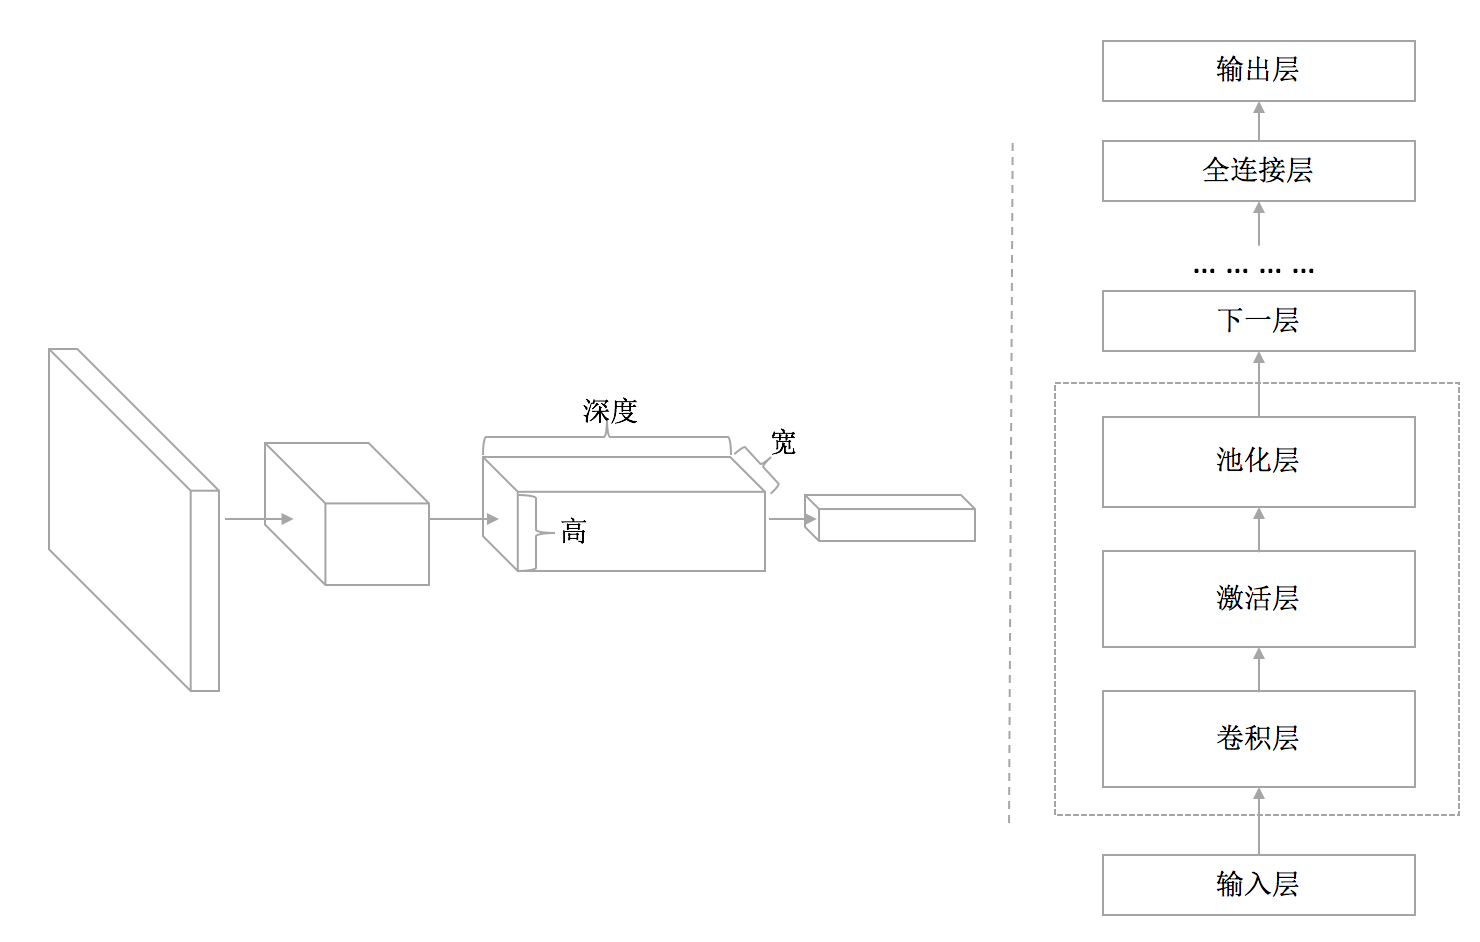
\includegraphics[scale=0.5]{figures/gan-cnn.png}
\caption{(左)卷积神经网络,(右)卷积神经网络的基本组织结构}
\label{fig:gan-cnn}
\end{figure}

图\ref{fig:gan-cnn}(左)是一个简单的4层卷积神经网络。卷积神经网的运算对象均表示为3维矩阵,令$[w, h, c]$表示宽为w,高为h,深为c的矩阵。比如一张像素为24*24的RGB彩色图片,可表示为[24, 24, 3],深度3表示RBG三色通道。

图\ref{fig:gan-cnn}(右)是卷积神经网络的基本结构。一次完整的卷积运算一般由卷积层(Convolutional Layer)、激活层(Active Layer)和池化层(Pooling Layer)叠加的基本单元完成(对应图中虚线框),更深的卷积神经网络是以上基本单元的叠加结果。卷积层实现提取局部特征的矩阵运算,激活层是激活函数非线性单元,池化层负责降采样。另外,全连接层(Fully Connected Layer)一般对应一个浅层全连接前馈神经网络,负责连接各局部特征,由此得到特征向量支持输出层完成分类、预测等机器学习任务。

(1)卷积层

卷积层进行卷积运算,以二维矩阵为例,如图\ref{fig:gan-cnn-ops},输入为3*4的矩阵$X$,卷积核为2*2的矩阵。卷积运算为,以与卷积核相同大小的矩阵为窗口(2*2的矩阵),从矩阵$X$的左上方开始,从左至右,从上至下滑动,每次从$X$截取窗口大小的区块(2*2矩阵),这样的区块通常称为感知域(reception filed),与卷积核进行卷积运算,即计算两个矩阵的点积(两个矩阵对应位置相乘再求和)。图\ref{fig:gan-cnn-ops}红色矩形对应第一次卷积运算过程。依次以1为步长,从左至右,从上至下滑动窗口并重复类似的卷积运算以完成余下的所有计算,最后得到一个二维矩阵输出,通常称为特征映射(Feature map)。此过程可形式化的定义为等式\ref{eq:gan-cnn-conv},$m,n$分别表示窗口的宽和高,$Z$为输出矩阵,$Z_{i,j}$表示$Z$在第$i$行,第$j$列的元素。

一般化到三维输入,令$X=[w, h, c]$表示宽为w,高为h,深为c的矩阵输入,对应的卷积核也是三维矩阵并且深度必须和输入的深度一致,表示为$K=[m, n, c]$。卷积运算过程为,以同$K$规模一样的窗口,并令步长为1,在$X$上进行滑窗计算,形式化的定义为等式\ref{eq:gan-cnn-conv-3d}。值得注意输出为二维矩阵。
\begin{equation}
\label{eq:gan-cnn-conv}
Z_{i,j} = (X*K)(i,j) = \sum_{m}\sum_{n}X_{i+m, j+n}K_{m,n}
\end{equation}
\begin{equation}
\label{eq:gan-cnn-conv-3d}
Z_{i,j} = (X*K)(i,j) = \sum_{m}\sum_{n}\sum_{d}X_{i+m, j+n,d}K_{m,n,d}
\end{equation}

卷积运算涉及的卷积核是需要学习的参数并且一次完整的卷积运算共享一个卷积核,因此卷积运算具有参数共享的性质,由此相比于全连接前馈网络大大减少了所需学习的参数量,进而更省空间。一次卷积运算需要一个卷积核,一个卷积核对应一个二维矩阵输出,通常一次这样的运算只能提取一种或一类特征。因此需要若干相同规模的卷积核进行多次卷积运算得以到多个对应不同类型特征的二维矩阵,最后将这些矩阵拼接可得到三维特征矩阵输出。

令$Z=[w_{z}, h_{z}, c_{z}]$表示输出的三维特征矩阵,其规模由卷积核个数、卷积核规模和滑窗运算步长(stride)共同决定。令$X=[w_{x}, h_{x}, c_{x}]$表示输入,$n_{f}$表示卷积核个数,$K=[w_{k},h_{k},c_{k}]$表示卷积核,$s$表示步长,那么$w_{z} = \left \lfloor (w_{x} - w_{k})/s \right \rfloor + 1, h_{z} = \left \lfloor (h_{x} - w_{k})/s \right \rfloor + 1, c_{z} = n_{f}$。

可以注意到除非$w_{k}=h_{k}=1$且$s=1$,否则输出规模必然小于输入规模。因此对于多层卷积神经网络,逐层进行以上卷积运算,特征矩阵很快就会缩小到无法计算的程度(当特征矩阵比卷积核还小时,无法继续进行运算)。如图\ref{fig:gan-cnn-padding}(左),以一维向量运算为例,卷积核大小为3,步长为1,特征向量从5个元素减少到3个元素,以此递减元素个数将很快减小到1。为了构建深度卷积神经网络,通常需要卷积操作的输出规模不要减小或减小得不那么急剧,由此引入了一个重要操作,即零填补(zero-padding),通常称为填补(padding)。padding在卷积运算前使用0来填充输入矩阵的边沿由此降低输出规模减小的速度。假设零填补填补参数为$p$,此时 $w_{z} = \left \lfloor (w_{x}+2p-w_{k})/s \right \rfloor + 1, h_{z} = \left \lfloor (h_{x}+2p-h_{k})/s \right \rfloor+1$。如图\ref{fig:gan-cnn-padding}(右),以一维向量运算为例,积核大小为3,步长为1,零填补参数为1(白色圈对应填补),由此保证输出规模与输入相同,进而支持多次类似运算得以实现。

通常卷积操作根据有无填补分为两种模式:(1)不使用填补操作,对应图\ref{fig:gan-cnn-padding}(左);(2)设置适当的填补参数$p$使得输出规模和输入规模相同,对应图\ref{fig:gan-cnn-padding}(右)。
% padding 有两种方式,一般称为same,valid。

\begin{figure}[H]
\centering
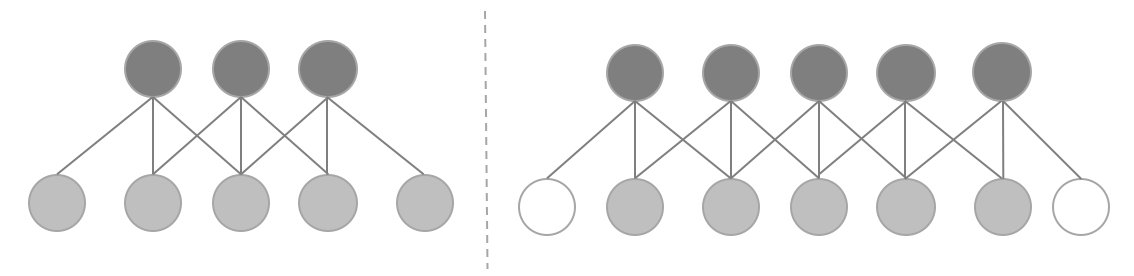
\includegraphics[scale=0.5]{figures/gan-cnn-padding.png}
\caption{(左)无填补的运算结果;(右)填补参数为1的运算结果}
\label{fig:gan-cnn-padding}
\end{figure}

(2) 激活层

激活层是使卷积神经网络具有非线性的关键,由激活函数构成,在卷积神经网络中通常使用ReLU激活函数及其变种,Sigmoid和Tanh只在输出层使用。如图\ref{fig:gan-cnn-ops},激活层对卷积层输出的特征矩阵的每一个元素进行激活运算,并将计算结果输入到池化层。

(3) 池化层

池化层主要的作用是降采样,同时池化操作可以让卷积神经网络具有不变式(invariant)特性。池化层运算的核心思想为,通过给定的滑动窗口进行规约运算,即使用一个统计值表示滑窗对应的区块,进而实现降维的目的。如图\ref{fig:gan-cnn-ops},以2*2的滑窗进行池化运算,图中蓝色框对应第一次运算,使用窗口对应区块内的最大值表示当前区块,依次从左往右、从上往下、以步长为1的方式滑动窗口重复进行以上运算,此过程通常称为最大池化(max pooling),常用的还有均值池化(average pooling)。一般的,假设输入$X=[w_{x}, h_{x}, c_{x}]$,滑窗大小为$[w_{p}, h_{p}]$,滑动步长为$s$,那么对于输出$Z=[w_{z}, h_{z}, c_{z}]$有,$w_{z} = \left \lfloor (w_{x}-w_{p})/s \right \rfloor+1, h_{z} = \left \lfloor (h_{x}-h_{p})/s \right \rfloor+1, c_{z}=c_{x}$。

(4)全连接层

 全连接层在卷积神经网络的最后一层,是浅层(通常是一层),全连接前馈网络,由此实现比如分类或回归等监督学习任务。在此之前,通常需要进行压平(flatten)操作将三维矩阵转换成向量的形式。

\begin{figure}[H]
\centering
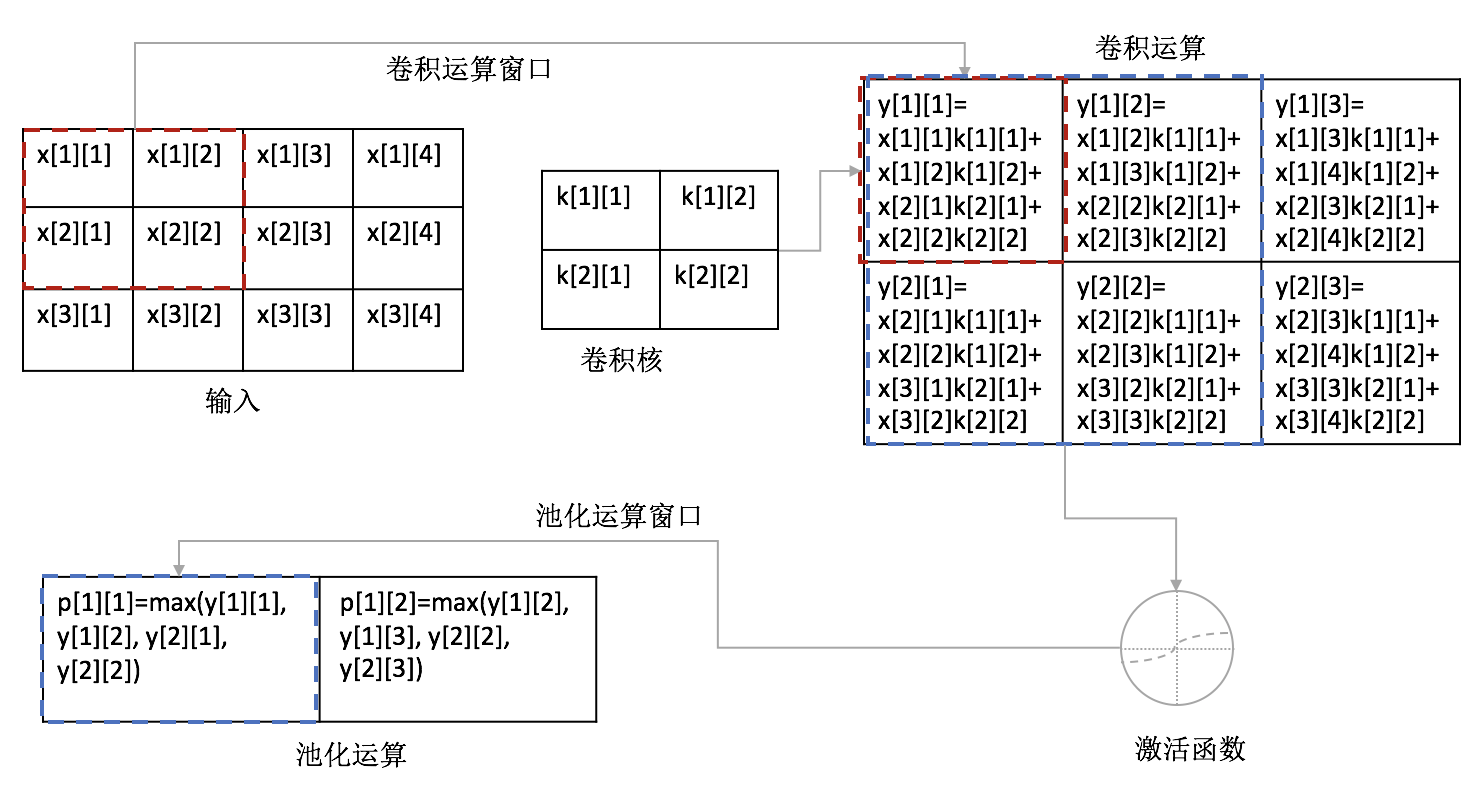
\includegraphics[scale=0.5]{figures/gan-cnn-ops.png}
\caption{卷积神经网络的一次卷积、激活和池化运算}
\label{fig:gan-cnn-ops}
\end{figure}

\section{模型与应用方案设计}

\subsection{时间序列生成式对抗网络 TSGAN}
% DCGAN:
% Replace any pooling layers with strided convolutions (discriminator) and fractional-strided convolutions (generator).
% Remove fully connected hidden layers for deeper architectures.
% Remove fully connected hidden layers for deeper architectures.
% Use ReLU activation in generator for all layers except for the output, which uses Tanh.
% Use LeakyReLU activation in the discriminator for all layers.
%
% Different Convolution operation
% 中文,介绍得还挺清楚:https://buptldy.github.io/2016/10/29/2016-10-29-deconv/
% An Introduction to different Types of Convolutions in Deep Learning: https://towardsdatascience.com/types-of-convolutions-in-deep-learning-717013397f4d
% Theano 的 tutorial, 似乎更详细:http://deeplearning.net/software/theano/tutorial/conv_arithmetic.html
%
% Batchnorm
% 原文【把原文batch-norm操作的算法copy过来就可以,说明优势】:https://arxiv.org/abs/1502.03167

本文针对普遍存在的时间序列数据结合卷积神经网络和生成式对抗网络提出时间序列生成式对抗网络(TSGAN)。TSGAN的生成器是一个卷积神经网络负责学习给定时间序列数据集的分布,如图\ref{fig:gan-ts-generator},基于噪音输入生成时间序列样本;TSGAN的判别器是由卷积神经网络构成的二分类器,如图\ref{fig:gan-ts-discriminator}所示,其输出为样本确实来自真实数据集的概率;TSGAN 的训练过程为生成器和判别器的博弈,算法\ref{gan-tsgan-algorithm},基于梯度下降和反向传播算法进行迭代更新。生成器以生成更真实的时间序列样本为目标,即最大化其生成样本在判别器中的输出概率;判别器以正确辨别样本真伪为目标,即最大化真实样本的输出概率同时最小化生成样本的输出概率。

(1)TSGAN的基本运算

TSGAN的核心由两个卷积神经网络构成,有关神经网络和卷积神经网络的通用计算可以参考前文介绍。这里主要介绍两个特殊运算,即小数跨步卷积(Fractional Strided Convolution, FSC)\cite{dosovitskiy2015learning}和批量归一化(Batch Normalization)\cite{ioffe2015batch}。

1. 小数跨步卷积

%Convolution: Convolution+Pooling; Deconvolution: Unpooling+Convolution。
小数跨步卷积,又可称转置卷积(Transpose Convolution)或反卷积(Deconvolution)。一般的卷积神经网络的运算顺序为先进行卷积运算然后进行池化运算;而小数跨步卷积可看成以上运算的逆过程,先进行反池化运算然后进行卷积运算。

令各维度的步长为$s$,输入$X=[w_{x}, h_{x}, c_{x}]$,输入$Z=[w_{z}, h_{z}, c_{z}]$。反池化运算的过程可描述为,首先将输入矩阵中的每个元素映射为$s*s$的区块,此区块的左上角存放原输入中对应的元素而其他位置补0,由此可以得到$w_{x}*h_{x}$个大小为$s*s$的区块,对这些区块进行拼接得到输出$Z$,容易得$w_{z}=w_{x}*s, h_{z} = h_{x}*s, c_{z}=c_{x}$,输出规模相比于输入规模扩大了$s$倍。池化的作用是降维,而反池化的作用是升维。如图\ref{fig:gan-unpooling}通过反池化操作实现对输入的两倍扩大。如图\ref{fig:gan-unpooling}(上),$s=2$,输入为$X=[2, 2, c_{x}]$,经过反池化操作后得到输出$Z=[4, 4, c_{z}]$,规模扩大2倍;如图\ref{fig:gan-unpooling}(下),$s=2$,输入为$X=[3, 3, c_{x}]$,经过反池化操作后得到输出$Z=[6, 6, c_{z}]$,规模扩大了2倍。

综上所述小数跨步卷积先进行反池化运算然后进行卷积运算,对于步长$s$,相当于扩大输入$s$倍并且完成局部特征提取。
%经过 unpooling 以后使用same模式的convolution就可以实现每次增加两倍的目标。以上操作称为deconv。

\begin{figure}[H]
\centering
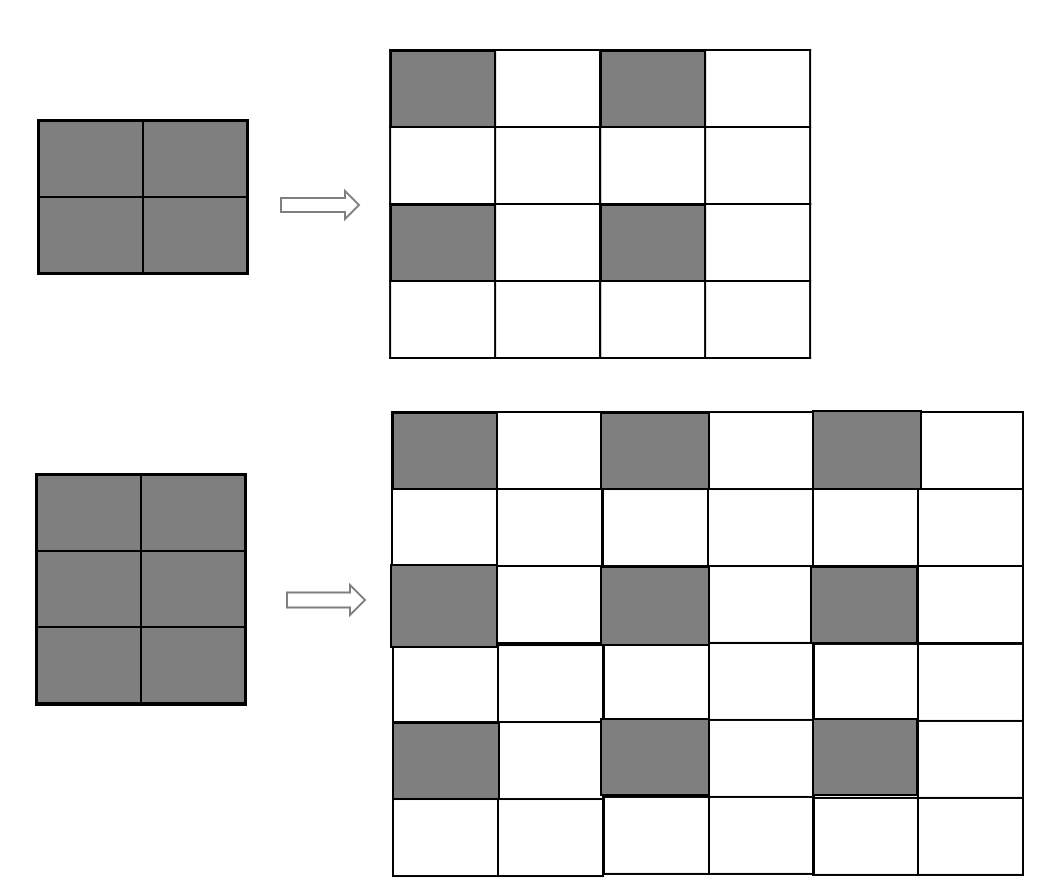
\includegraphics[scale=0.5]{figures/gan-unpooling.png}
\caption{反池化运算}
\label{fig:gan-unpooling}
\end{figure}

2. 批量归一化

批量归一化是对每次训练的小批样本进行归一化的操作,其优势为:可以让训练更简单高效,可以使用更大的学习率做为初始值、使模型对初始值不再那么敏感、可以作为规范化操作、在一定程度上可以避免使用dropout、收敛速度加快。具体的,对于每个小批量输入,先通过\ref{equ:gan-batchnorm-mean}等式计算样本均值、通过\ref{equ:gan-batchnorm-std}等式计算样本标准差,然后通过等式\ref{equ:gan-batchnorm-x}对输入进行规范化,最后通过等式\ref{equ:gan-batchnorm-out}计算返回值。
\begin{subequations}
\begin{align}
\mu_{B} &= \frac{1}{m}\sum_{i=1}^{m}x^{(i)}\label{equ:gan-batchnorm-mean}\\
\sigma_{B}^{2} &= \frac{1}{m}\sum_{i=1}^{m}(x^{(i)}-\mu_{B})^{2} \label{equ:gan-batchnorm-std}\\
\hat{x}^{(i)} &= \frac{x^{(i)}-\mu_{B}}{\sqrt{\sigma_{B}^{2}+\epsilon }} \label{equ:gan-batchnorm-x}\\
z^{(i)} &= \gamma \hat{x}^{(i)} + \beta \label{equ:gan-batchnorm-out}
\end{align}
\end{subequations}

 (2)TSGAN的生成器

图\ref{fig:gan-ts-generator}是TSGAN的生成器的结构。输入为随机产生的一维噪音向量$z$,其长度为$0.7*n$,其中$n$表示真实数据集中时间序列的长度(采样点个数)。首先通过变形或映射操作将输入转成3维矩阵,然后经过4层小数跨步卷积运算得到最后的输出,输出是长度为$n$的生成样本。其中每一次小数跨步卷积运算会进行批量归一化运算,隐藏层的激活函数为ReLU,输出层为线性单元。卷积核统一为1*5规模,步长统一为2,每一次小数跨步卷积运算实现2倍的升维。
% 最后输出层必须是线性单元!很关键!

\begin{figure}[H]
\centering
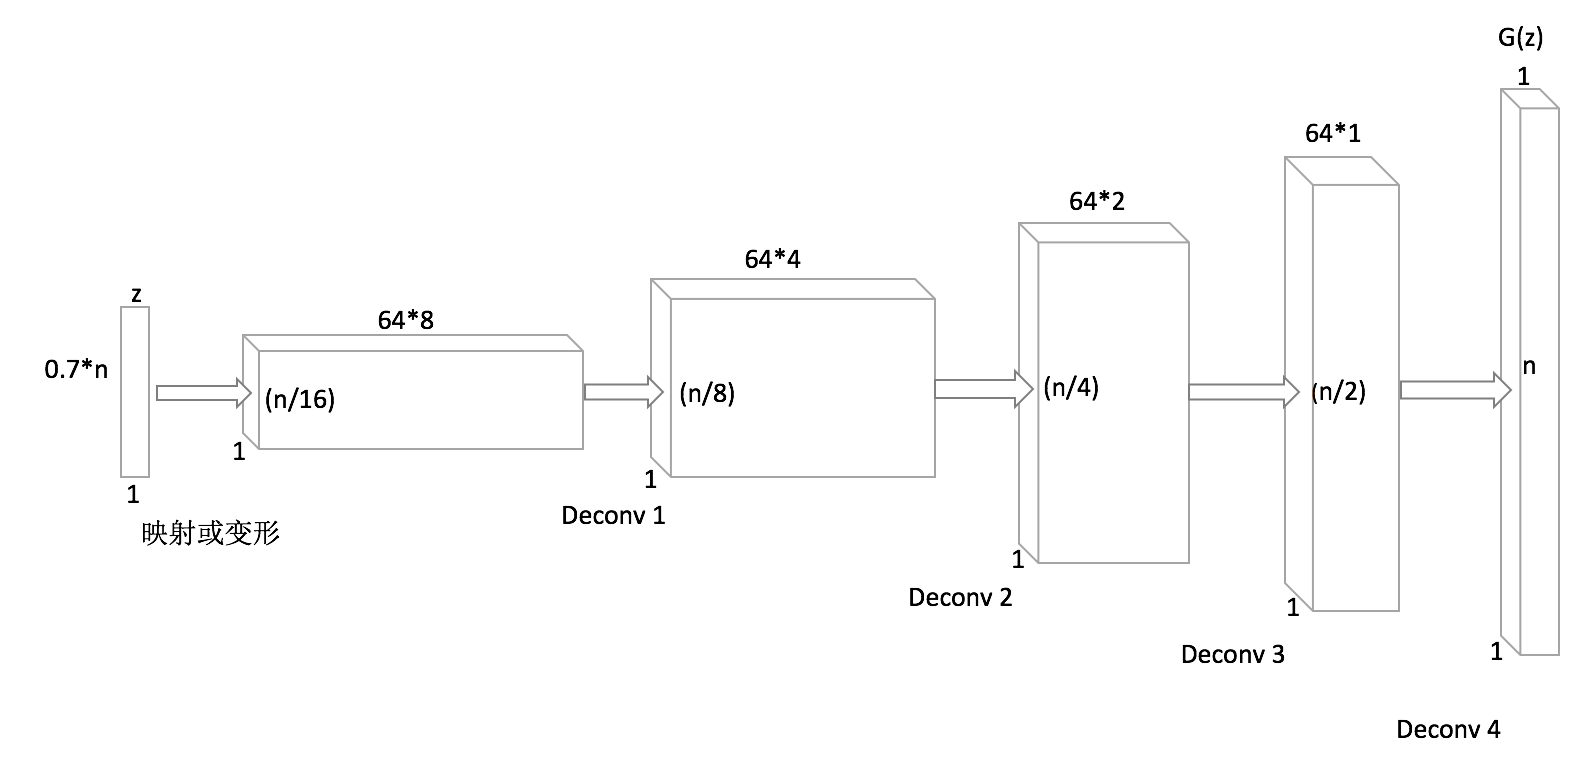
\includegraphics[scale=0.5]{figures/gan-ts-generator.png}
\caption{TSGAN 的生成器}
\label{fig:gan-ts-generator}
\end{figure}

(3)TSGAN的判别器

图\ref{fig:gan-ts-discriminator}是TSGAN的判别器。对输入长度为$n$的样本,通过4层卷积层,最后通过压平(flatten)操作得到一维特征向量,最后使用Sigmoid作为输出层实现二分类,输出是样本为真的概率。网络中不使用任何池化操作,降维是通过无填补操作的卷积运算实现的。所有隐藏层使用LeakyReLU作为激活函数,并且卷积运算后进行批量归一化。卷积核统一为1*5规模,步长统一为2,每一次卷积运算实现2倍的降维。

\begin{figure}[H]
\centering
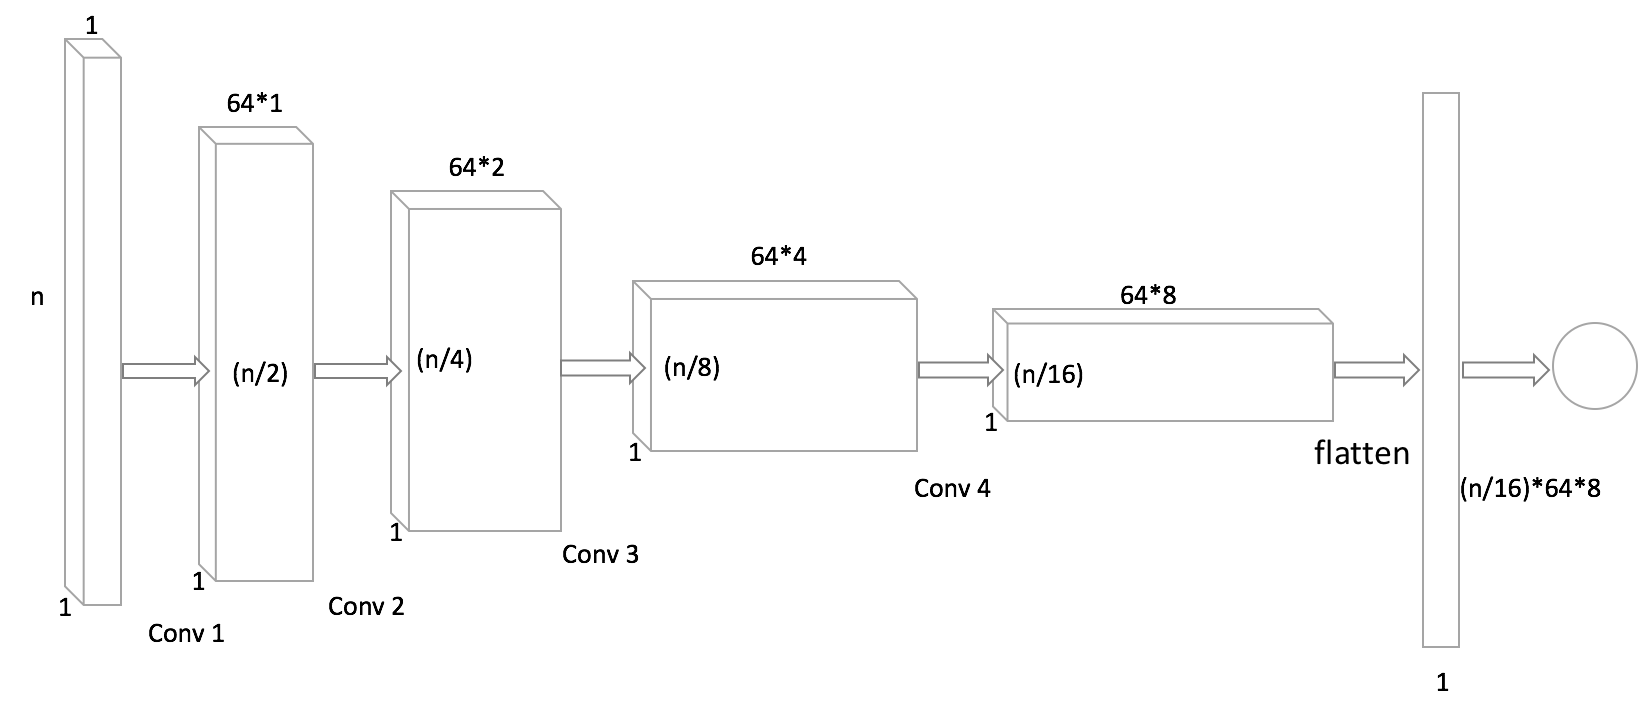
\includegraphics[scale=0.5]{figures/gan-ts-discriminator.png}
\caption{TSGAN 的判别器}
\label{fig:gan-ts-discriminator}
\end{figure}


(4)TSGAN的训练

\begin{algorithm}[H]
 \caption{基于随机梯度下降算法训练TSGAN}
 \KwData{生成器的更新次数gk,判别器的更新次数dk,训练迭代次数 epoch}
 \For{i=0; i<epoch; i++}{
  \For{j=0; j<dk; j++}{
    \ 从$p_{g}(z)$先验分采样 $\{z^{(1)}, ...., z^{(m)}\}$\;
    \ 从真实样本$p_{data}(x)$中采样,$\{x^{(1)}, ..., x^{(m)}\}$\; 
    \ 基于梯度下降算法更新判别器:$\bigtriangledown _{\theta_{d}} -\frac{1}{m}\sum_{i=1}^{m}[log(D(x^{(i)})) + log(1-D(G(z^{(i)})))]$
  }
  \For{j=0; j<gk; j++}{
    \ 从$p_{g}(z)$先验分采样 $\{z^{1}, ...., z^{m}\}$\;
    \ 基于梯度下降算法更新生成器:$\bigtriangledown _{\theta_{g}} -\frac{1}{m}\sum_{i=1}^{m}log(D(G(z^{i})))$ \;
  }
 }
 \renewcommand{\algorithmcfname}{算法}
 \label{gan-tsgan-algorithm}
\end{algorithm}

(5)TSGAN的评估

本文采用最近邻距离(Nearest Neighbour Distance, NND)和最大平均差异(Maximum Mean Discrepancy, MMD)来度量生成器生成时间序列样本的质量,两个指标的核心都是度量真实数据集和生成数据集的相似程度\cite{esteban2017real},指标都是越小越好。

1. 最近邻距离(NND)

(a)生成大量时间序列形成生成数据集;(b)计算每个生成时间序列到真实数据集的距离,具体为从真实数据集中找到离当前生成时间序列最近的序列并以它们之间的距离作为生成时间序列到真实数据集的距离;(c)对所有生成时间序列到真实数据集的距离进行平均,平均值表示生成数据集到真实数据集的距离,其值越小表明两个数据集越相似,进而说明生成器生成的时间序列质量越好。

2. 最大平均差异(MMD)

生成式对抗网络的本质是学习数据的分布,因此通过度量生成数据集和真实数据集分布的相似性可以反映生成器生成数据的质量。MMD 通过度量两个数据集统计信息的差异的平方(表示为$MMD^{2}$)来衡量两个数据集的距离,并且将两个样本之间的点积替换成核函数。假设有核函数$K: X \times Y \rightarrow \mathbb{R}$,以及两个大小分别为$m$和$n$的数据集$\{x^{(1)},x^{(2)},...,x^{(m)}\}, \{y^{(1)},y^{(2)},...,y^{(n)}\}$,那么$MMD^{2}$的无偏估定义如等式\ref{equ:gan-metrics-mmd},其中核函数使用基于L2距离的径向积函数(Radial Basis Function, RBF),即$K(x, y) = exp(-\left \| x-y \right \|^{2} / (2\sigma ^{2}))$。
\begin{equation}
\hat{MMD}^{2} = \frac{1}{n(n-1)}\sum_{i=1}^{n}\sum_{j\neq i}^{n}K(x_{i}, x_{j}) - \frac{2}{mn}\sum_{i=1}^{n}\sum_{j=1}^{m}K(x_{i}, y_{j}) + \frac{1}{m(m-1)}\sum_{i=1}^{m}\sum_{j\neq i}^{m}K(y_{i}, y_{j}) \label{equ:gan-metrics-mmd} 
\end{equation}

\subsection{基于TSGAN 的半监督式学习框架}

基于 TSGAN 本文构建了半监督式学习框架。TSGAN 通过无监督的方式进行训练后,一方面生成器可以学习真实数据集的分布,可作为模拟器用于数据生成;另一方面判别器可作为特征转换器(类似于自动自编码机的编码器)与监督式学习融合形成半监督式学习框架,支持分类,预测、聚类、切割、索引、异常检测和主题发现等机器学习任务,本文以时间序列分类任务作为应用。

图\ref{fig:gan-semi-supervised-learning}是基于TSGAN判别器的半监督式学习框架。TSGAN的判别器总共有4次卷积操作,每次卷积操作都产生一个特征矩阵,本文对后3个特征矩阵进行应用,丢弃第1个低维特征。直接拼接以上特征矩阵维度过高,因此本文将每一个特征矩阵接入池化层并通过最大池化操作对特征进行规约。

首先,基于层次越深特征抽象层次越高特征越有价值的启发式认识,假设特征矩阵的高度为$h$,对于从浅到深的三个特征矩阵,本文依次使用大小为 $h/2$, $h/3$, $h/4$ 的滑窗进行最大池化规约运算。然后通过压平操作将特征矩阵转换成一维特征向量。最后将三个特征向量进行拼接形成样本新的表示。

本文将通过以上操作获取的特征向量输入到基于欧式距离的1近邻(ED-1NN)、基于线性核函数的支持向量机(LinearSVM)和逻辑斯蒂回归(LR)简单分类器中实现时间序列分类任务。值得一提的是,本文采用简单分类器是为了体现TSGAN所提特征的有效性,ED-1NN是时间序列分类任务的基线、LinearSVM和LR通常是验证无监督式特征学习效果的通用基线。

\begin{figure}[H]
\centering
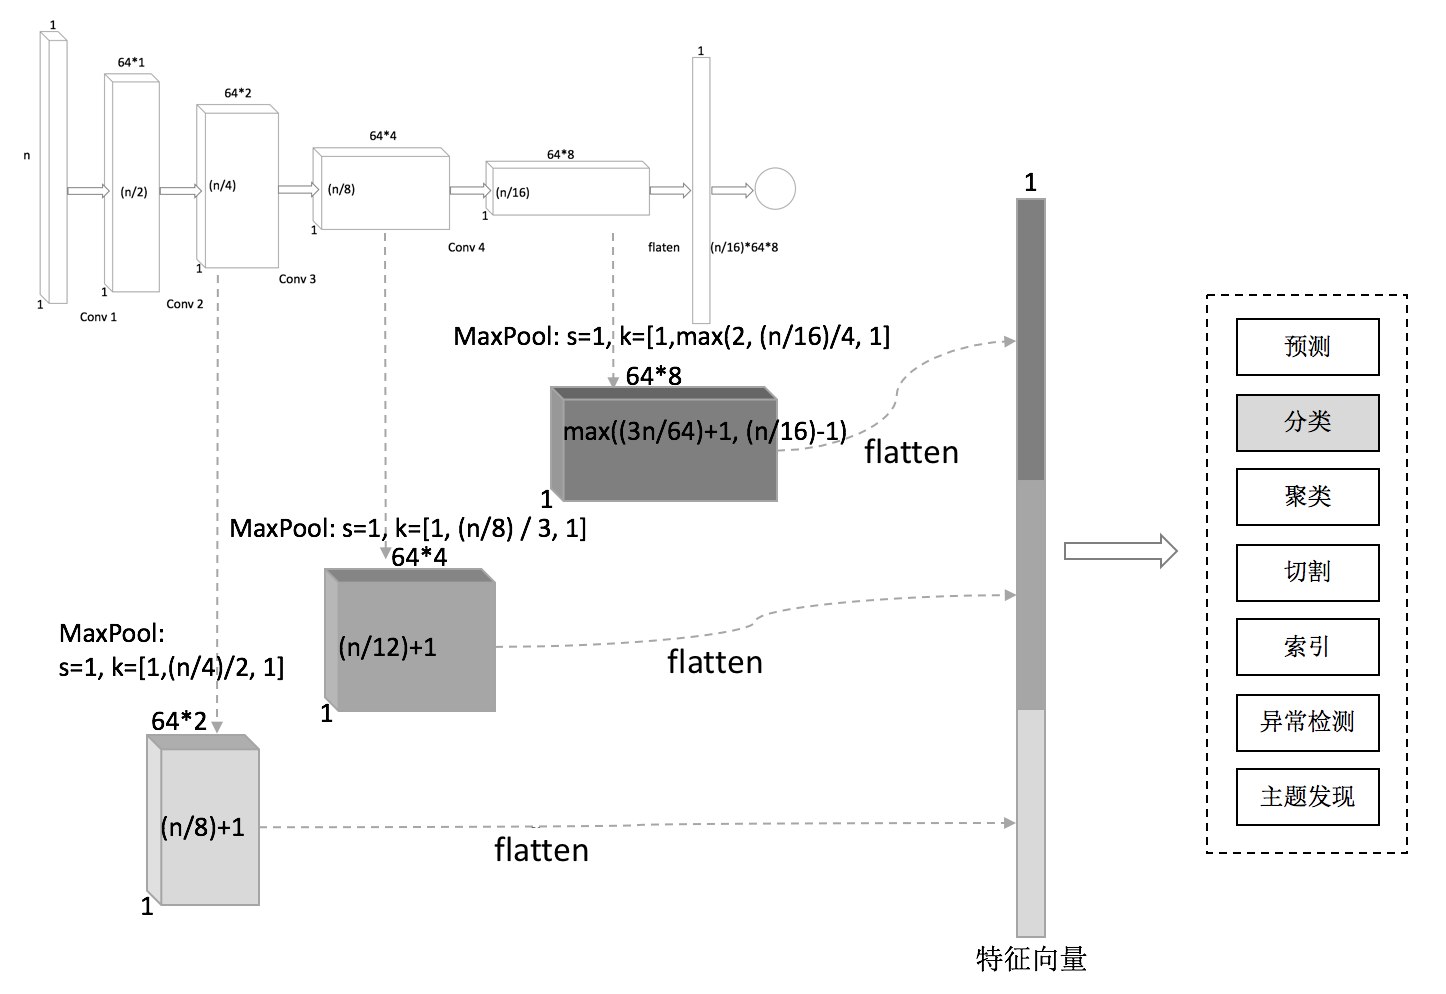
\includegraphics[scale=0.6]{figures/gan-semi-supervised-learning.png}
\caption{TSGAN的判别器作为特征转换器形成的半监督式学习框架}
\label{fig:gan-semi-supervised-learning}
\end{figure}

假设有训练集$Train = \{(x^{(1)}, y^{(1)}), (x^{(2)}, y^{(2)}), ..., (x^{(m)}, y^{(m)})\}$和测试集$Test = \{(x^{(1)}, y^{(1)}), (x^{(2)}, y^{(2)}), ..., (x^{(n)}, y^{(n)})\}$

(1)ED-1NN 分类算法

ED-1NN 分类算法没有训练过程,对于每个测试样本$(x,y)$的预测可分为两步:(a)计算$x$到训练集中每个样本的距离,即$d^{(i)} = \left \| x-x^{(i)} \right \|^{2},i=1,2,...,m$;(b)计算$x$的预测值$\hat{y}$,$\hat{y}$是距离最近的训练样本对应的类标,即$\hat{y}=y^{(i)}=argmin_{i \in \{1,2,...,m\}}d^{(i)}$。

重复以上两个步骤$n$次即可获得所有测试样本的估计值。

(2)LinearSVM

标准的LinearSVM是一个二分类器,其损失函数为$J(\theta) = \lambda\sum_{1}^{m}max(0, 1-y^{(i)}(w^{T}x^{(i)}+b)) +  \frac{1}{2}\left \| w \right \|^{2}$,其中$\lambda$为惩罚因子。

对于多分类问题,假设有$C$个类,对每个类$c \in \{1,2,...,C\}$训练一个标准LinearSVM二分类器,由此得到$C$个二分类器分别对应的$C$组参数,即$\{(w^{(1)}, b^{(1)}), (w^{(2)}, b^{(2)}), ...., (w^{(C)}, b^{(C)})\}$。那么预测的估计值为$\hat{y} = argmax_{c}((w^{(c)})^{T}x+b^{(c)})$

(3)逻辑斯蒂回归(LR)

标准的LR是二分类器,对于任意样本$(x,y)$,其中$y \in {0,1}$,0表示负例,1表示正例,LR的训练过程如下:(a) LR根据等式$h_{\theta}(x) = \frac{1}{1+e^{-\theta^{T}x}}, h_{\theta}(x) = [0,1]$计算每个样本$x$为正例的概率;(b) LR根据损失函数$J(\theta) = -\frac{1}{m}[\sum_{1}^{m}y^{(i)}log(h_{\theta}(x^{(i)}))+(1-y^{(i)})log(1-h_{\theta}(x^{(i)}))] + \frac{1}{2}\left \| \theta \right \|^{2}$ 训练模型。(c)在预测阶段,对每个样本x计算其属于正样本的概率$h_{\theta}(x^{(i)}), i=1,...n$,如果概率大于等于0.5,则预测类标为1,否则为0。

对于多分类问题,假设有$C$个类。对每个类$c \in \{1,2,...,C\}$训练一个二分类器$ h_{\theta}^{c}(x)$,此时所有$y=c$的样本都为正例,其他样本都被看作是负例。预测时,$ \hat{y} = argmax_{c} h_{\theta}^{c}(x)$,即$C$个分类器中输出概率最大的那个分类器的类标将作为当前样本的预测值。

(4)分类效果评估

通过分类准确率来衡量分类的效果,具体定义为$acc = \frac{1}{m}\sum_{i=1}^{m}\mathbb{I}(h(x^{(i)}) = y^{(i)})$,其中$\mathbb{I}$为指示函数,当传入的表达式为真时取值为1,否则取值为0。


\section{实验结果及分析}

本文使用最大的时间序列分类公开数据集UCR\cite{bagnall16bakeoff}进行实验。UCR总共包含85个时间序列数据集,每个数据集都是由若干类别的单元时间序列构成。本文根据数据特性,将UCR数据集划分为以下几类:基于加速计采集的运动时间序列数据集、基于形状的时间序列数据集、基于传感器采集的频谱时间序列数据集、医疗时间序列数据集和工业系统时间序列数据集。

本文通过TensorFlow实现模型,并采用统一配置参数。模型参数参考前文的模型设计。训练参数,本文采用Adam梯度下降算法,生成器和判别器的初始学习率都是0.0002,训练迭代次数为200。训练集和测试集的划分和公开数据集的划分一致。

(1)TSGAN生成时间序列效果展示

值得注意的是,虽然数据集有类标记,但为了体现TSGAN对无标记数据的学习能力,本文训练过程均采用无监督式学习。对每个时间序列数据集,采用NND和MMD指标评估生成样本的质量,计算基于100000个时间序列生成样本和各自的真实测试样本。通过大量实验充分证明TSGAN的生成器可有效学习时间序列数据集的分布并生成逼真的多样化的时间序列。由于数据集较多,本文每一类数据集展示一组示例。

1. 基于传感器采集的频谱时间序列数据集。如图\ref{fig:gan-show-InsectWingbeatSound}为数据集InsectWingbeatSound的生成结果。InsectWingbeatSound是通过传感器采集的昆虫振翅声的功率频谱,是11类雄性和雌性蚊子的采样结果。

2. 基于形状的时间序列数据集。如图\ref{fig:gan-show-ArrowHead}为数据集ArrowHead的生成结果,ArrowHead是通过极坐标将三类箭头图片影射而成的时间序列。
%基于形状的时间序列是一种典型的数据类型,通过某种映射方式将图片、文字等物体影射为一维时间序列。

3. 基于加速计采集的运动时间序列数据集。如图\ref{fig:gan-show-uWaveGestureLibrary_Z}为数据集uWaveGestureLibrary\_Z的生成结果。uWaveGestureLibrary\_Z是通过加速计采集的8类手势运动数据。

4. 医疗时间序列数据集。如图\ref{fig:gan-show-ECGFiveDays}为数据集ECGFiveDays的生成结果,是2类心电图信号。

5. 工业系统时间序列数据集。如图\ref{fig:gan-show-FordA}为数据集FordA的生成结果。FordA是汽车子系统运行状态下的引擎噪音信号,是2008年电气和电子工程师协会(Institute of Electrical and Electronics Engineers, IEEE)计算智能世界大会的时间序列分类竞赛数据集。竞赛任务为识别某种特定症状是否存在于汽车子系统中,因此FordA包含两类时间序列(正常数据和故障数据),是典型的故障分类问题。
%This data was originally used in a competition in the IEEE World Congress on Computational Intelligence, 2008. The classification problem is to diagnose whether a certain symptom exists or does not exist in an automotive subsystem. Each case consists of 500 measurements of engine noise and a classification. There are two separate problems: For FordA the Train and test data set were collected in typical operating conditions, with minimal noise contamination.

% spectrograms
\begin{figure}[H]
\centering
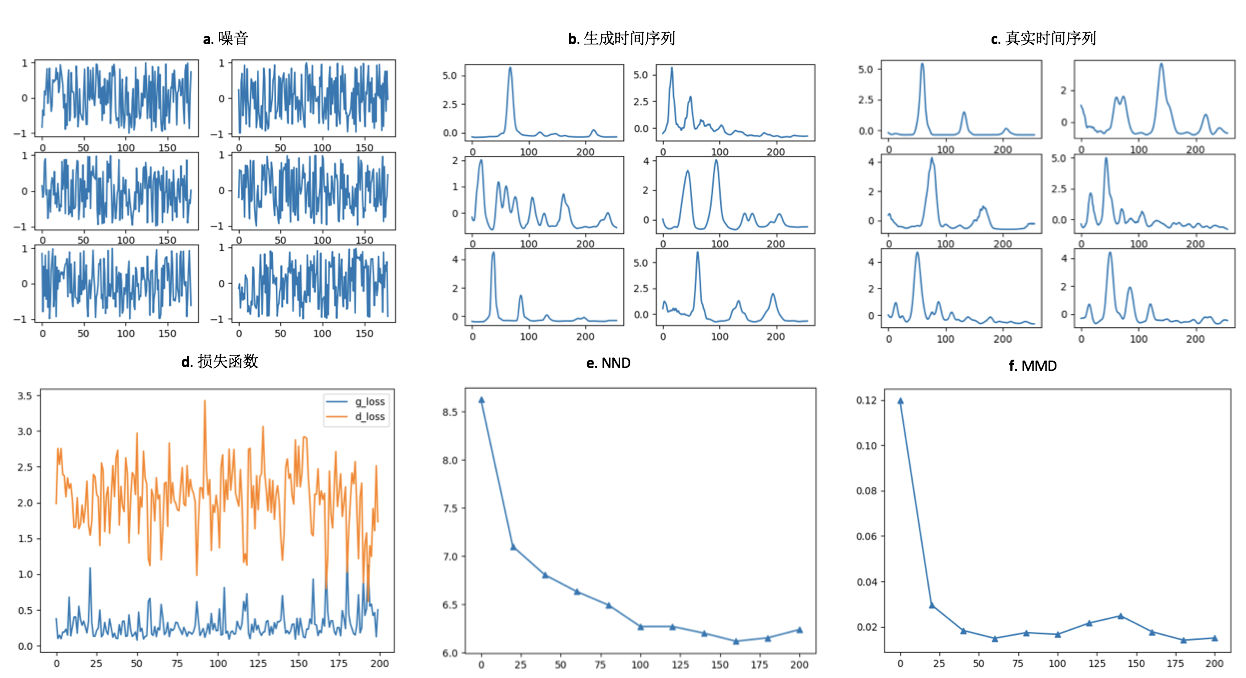
\includegraphics[scale=0.5]{figures/gan/InsectWingbeatSound.png}
\caption{InsectWingbeatSound 数据集的生成结果}
\label{fig:gan-show-InsectWingbeatSound}
\end{figure}
% Shape
\begin{figure}[H]
\centering
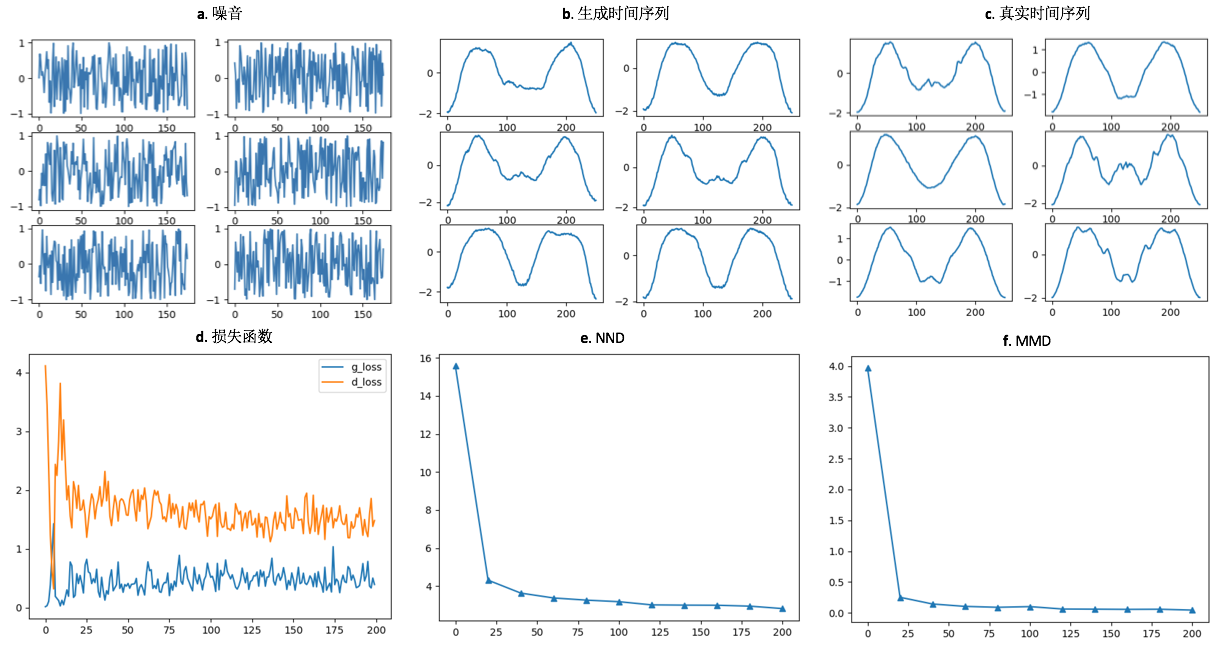
\includegraphics[scale=0.5]{figures/gan/ArrowHead.png}
\caption{ArrowHead 数据集的生成结果}
\label{fig:gan-show-ArrowHead}
\end{figure}
% accelerometers ---- motion
\begin{figure}[H]
\centering
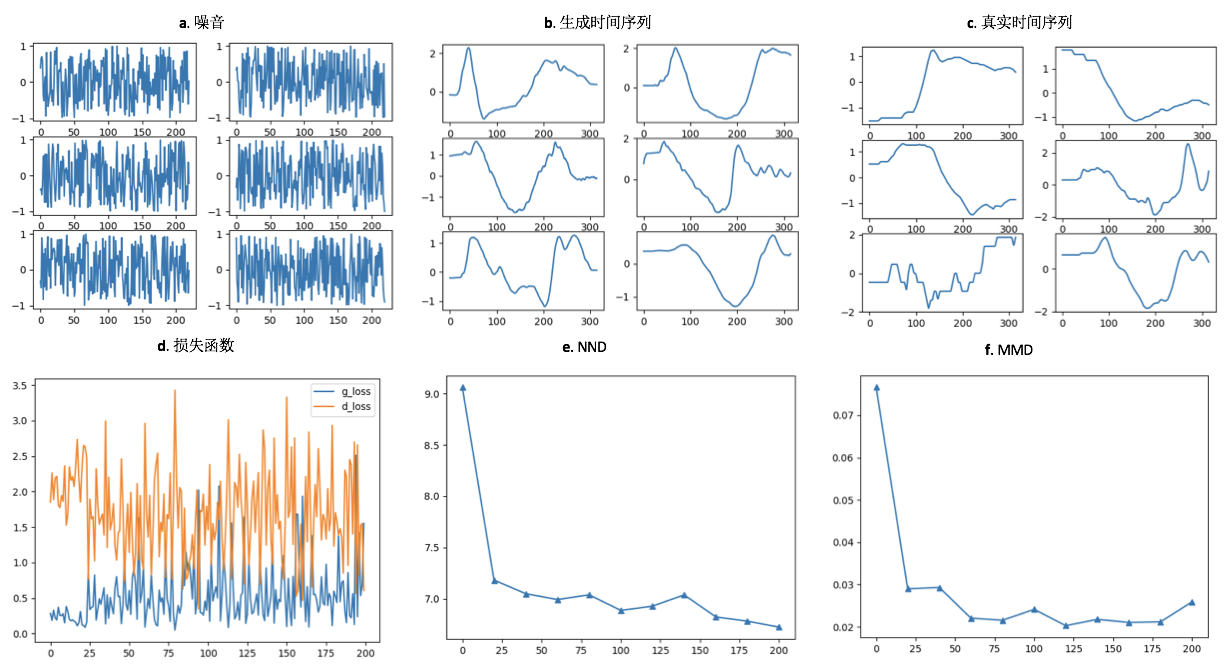
\includegraphics[scale=0.5]{figures/gan/uWaveGestureLibrary_Z.png}
\caption{uWaveGestureLibrary\_Z 数据集的生成结果}
\label{fig:gan-show-uWaveGestureLibrary_Z}
\end{figure}
% ECG
\begin{figure}[H]
\centering
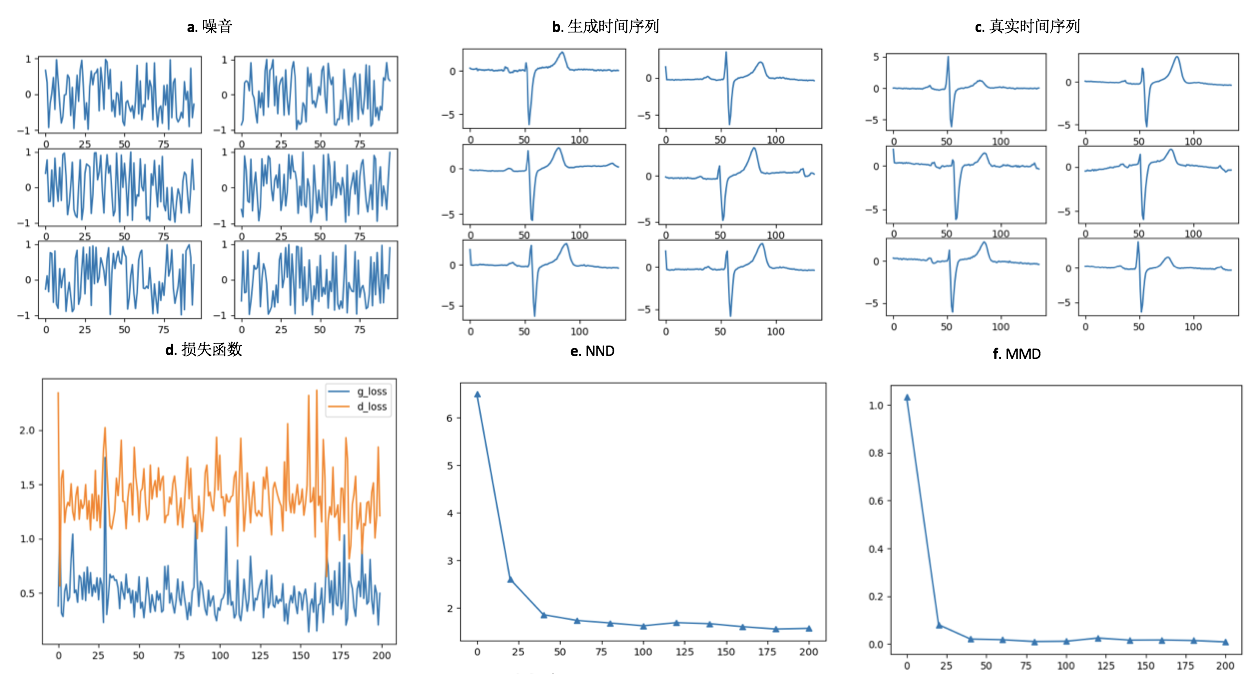
\includegraphics[scale=0.5]{figures/gan/ECGFiveDays.png}
\caption{ECGFiveDays 数据集的生成结果}
\label{fig:gan-show-ECGFiveDays}
\end{figure}
% Device
\begin{figure}[H]
\centering
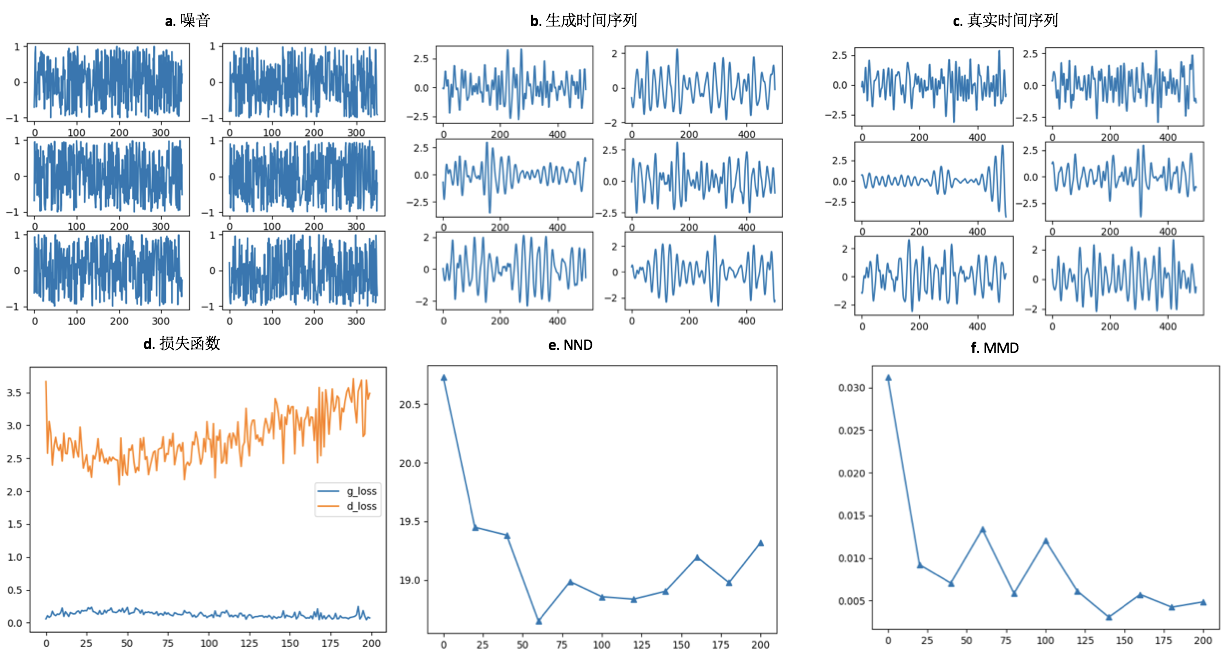
\includegraphics[scale=0.5]{figures/gan/FordA.png}
\caption{FordA 数据集的生成结果}
\label{fig:gan-show-FordA}
\end{figure}

(2)基于TSGAN的半监督式时间序列分类结果

本文将利用无标记数据训练好的TSGAN的判别器作为特征转换器与ED-1NN,LinearSVM和LR分类器结合形成半监督式时间序列分类框架。表\ref{tab:gan-classify}对比是否有TSGAN特征转换器的分类效果,可以看到有TSGAN特征转换器的分类准确率更高。图\ref{fig:gan-acc-knn},从左至右依次对应ED-1NN,LinearSVM和LR的分类对比结果,横坐标为基于原生时间序列的分类准确率,纵坐标为基于TSGAN特征转换器获取的特征向量的分类准确率,可以看到绝大部分的数据集都位于对角线上方,说明基于TSGAN特征转换器获取的特征向量的分类效果更好。以上结果充分说明TSGAN基于无标记数据可以学习数据关键特征。

\begin{longtable}[c]{p{5cm}*{6}{c}}
\caption{分类结果}\label{tab:gan-classify}\\
\toprule[1.5pt]
数据集 & \multicolumn{2}{c}{1NN} & \multicolumn{2}{c}{LSVC} & \multicolumn{2}{c}{LR} \\
    & \multicolumn{1}{c}{原数据} & \multicolumn{1}{c}{GAN特征}& \multicolumn{1}{c}{原数据}& \multicolumn{1}{c}{GAN特征}& \multicolumn{1}{c}{原数据}&  \multicolumn{1}{c}{GAN特征} \\\midrule[1pt]
\endfirsthead
\multicolumn{7}{c}{续表~\thetable\hskip1em 分类结果}\\
\toprule[1.5pt]
数据集 & \multicolumn{2}{c}{1NN} & \multicolumn{2}{c}{LSVC} & \multicolumn{2}{c}{LR} \\
  & \multicolumn{1}{c}{原数据} & \multicolumn{1}{c}{GAN特征}& \multicolumn{1}{c}{原数据}& \multicolumn{1}{c}{GAN特征}& \multicolumn{1}{c}{原数据}&  \multicolumn{1}{c}{GAN特征} \\\midrule[1pt]
\endhead
\hline
\multicolumn{7}{r}{续下页}
\endfoot
\endlastfoot
50words &0.6308 &0.7297 &0.5011 &0.7758 &0.5341 &0.7758 \\
Adiac &0.6113 &0.7289 &0.6189 &0.7545 &0.6752 &0.79780 \\
ArrowHead &0.8000 &0.8286 &0.6743 &0.8 &0.765 &0.8171 \\
Beef &0.6667 &0.6000 &0.8667 &0.8333 &0.8667 &0.8333 \\
BeetleFly &0.7500 &0.6500 &0.8000 &0.8000 &0.8500 &0.8000 \\
BirdChicken &0.5500 &0.7000 &0.7500 &0.8000 &0.7500 &0.9000 \\
CBF &0.8522 &1.0000 &0.7122 &0.9944 &0.8344 &0.9944 \\
Car &0.7333 &0.7167 &0.8167 &0.8333 &0.8667 &0.8333 \\
ChlorineConcentration &0.6500 &0.8456 &0.7221 &0.9070 &0.8240 &0.9010 \\
CinC\_ECG\_torso &0.8971 &0.8913 &0.4551 &0.9072 &0.4964 &0.9275 \\
Coffee &1.0000 &1.0000 &1.0000 &1.0000 &1.0000 &1.0000 \\
Computers &0.5760 &0.5320 &0.5120 &0.6360 &0.5080 &0.6560 \\
Cricket\_X &0.5769 &0.6487 &0.2333 &0.7077 &0.2974 &0.7205 \\
Cricket\_Y &0.5667 &0.6513 &0.2333 &0.7410 &0.3692 &0.7462 \\
Cricket\_Z &0.5872 &0.6410 &0.2231 &0.7103 &0.2949 &0.7205 \\
DiatomSizeReduction &0.9346 &0.9542 &0.9706 &0.9706 &0.9608 &0.9608 \\
DistalPhalanxOutlineAgeGroup &0.7825 &0.7550 &0.7825 &0.7450 &0.8000 &0.8250 \\
DistalPhalanxOutlineCorrect &0.7517 &0.7750 &0.6967 &0.7983 &0.7000 &0.8300 \\
DistalPhalanxTW &0.7275 &0.7125 &0.7500 &0.7475 &0.7650 &0.7875 \\
ECG200 &0.8800 &0.9200 &0.8500 &0.8900 &0.8500 &0.8900 \\
ECG5000 &0.9249 &0.9251 &0.9340 &0.9427 &0.9418 &0.9464 \\
ECGFiveDays &0.7967 &0.7758 &0.9431 &0.8177 &0.9547 &0.8177 \\
Earthquakes &0.6739 &0.6894 &0.5963 &0.7733 &0.6087 &0.7888 \\
ElectricDevices &0.5487 &0.6159 &0.4526 &0.6571 &0.4643 &0.6866 \\
FISH &0.7829 &0.8343 &0.8686 &0.9314 &0.8571 &0.9257 \\
FaceAll &0.7136 &0.7385 &0.7787 &0.8089 &0.8118 &0.8041 \\
FaceFour &0.7841 &0.8409 &0.8750 &0.8750 &0.8636 &0.8864 \\
FacesUCR &0.7693 &0.8951 &0.7307 &0.9283 &0.7512 &0.9259 \\
FordA &0.6590 &0.8259 &0.4957 &0.9145 &0.5062 &0.9234 \\
FordB &0.5578 &0.8045 &0.4978 &0.8914 &0.5072 &0.9109 \\
Gun\_Point &0.9133 &0.9600 &0.8467 &0.9667 &0.8467 &0.9867 \\
Ham &0.6000 &0.5619 &0.6095 &0.6952 &0.7429 &0.7238 \\
HandOutlines &0.8010 &0.8280 &0.8430 &0.8680 &0.8590 &0.8790 \\
Haptics &0.3701 &0.3734 &0.3929 &0.4968 &0.4643 &0.5260 \\
Herring &0.5156 &0.5156 &0.6250 &0.6250 &0.6875 &0.6406 \\
InlineSkate &0.3418 &0.3327 &0.2291 &0.3618 &0.2782 &0.3655 \\
InsectWingbeatSound &0.5616 &0.4424 &0.5263 &0.6121 &0.6409 &0.6268 \\
ItalyPowerDemand &0.9553 &0.9514 &0.9708 &0.9417 &0.9689 &0.9582 \\
LargeKitchenAppliances &0.4933 &0.5813 &0.3413 &0.7013 &0.3867 &0.7040 \\
Lighting2 &0.7541 &0.7213 &0.6393 &0.6885 &0.6721 &0.6885 \\
Lighting7 &0.5753 &0.6849 &0.5068 &0.6712 &0.6164 &0.7260 \\
MALLAT &0.9143 &0.8938 &0.8874 &0.9156 &0.8823 &0.9326 \\
Meat &0.9333 &0.9333 &0.9667 &0.9667 &0.9833 &0.96667 \\
MedicalImages &0.6842 &0.6500 &0.6092 &0.6513 &0.6184 &0.7342 \\
MiddlePhalanxOutlineAgeGroup &0.7400 &0.7325 &0.7650 &0.7725 &0.8050 &0.7975 \\
MiddlePhalanxOutlineCorrect &0.7533 &0.7700 &0.5333 &0.7933 &0.5400 &0.8067 \\
MiddlePhalanxTW &0.5614 &0.5664 &0.6216 &0.6040 &0.6441 &0.6391 \\
MoteStrain &0.8786 &0.8299 &0.8634 &0.8610 &0.8658 &0.8674 \\
NonInvasiveFatalECG\_Thorax1 &0.8290 &0.8753 &0.9094 &0.94402 &0.9160 &0.9466 \\
NonInvasiveFatalECG\_Thorax2 &0.8799 &0.8794 &0.9328 &0.93893 &0.9399 &0.9425 \\
OSULeaf &0.5207 &0.7355 &0.4463 &0.8636 &0.4669 &0.8636 \\
OliveOil &0.8667 &0.8667 &0.5667 &0.1667 &0.8667 &0.8667 \\
PhalangesOutlinesCorrect &0.7611 &0.7984 &0.6702 &0.8030 &0.6702 &0.8333 \\
Phoneme &0.1092 &0.2964 &0.0854 &0.3412 &0.09388 &0.3518 \\
Plane &0.9619 &0.9714 &0.9905 &0.9810 &0.9905 &0.9905 \\
ProximalPhalanxOutlineAgeGroup &0.7854 &0.8244 &0.8439 &0.8244 &0.8634 &0.8585 \\
ProximalPhalanxOutlineCorrect &0.8076 &0.8316 &0.8247 &0.4742 &0.8454 &0.9003 \\
ProximalPhalanxTW &0.7075 &0.7300 &0.7900 &0.7600 &0.8050 &0.8075 \\
RefrigerationDevices &0.3947 &0.5227 &0.3520 &0.5307 &0.3680 &0.5440 \\
ScreenType &0.3600 &0.3573 &0.3733 &0.3920 &0.3947 &0.4160 \\
ShapeletSim &0.5389 &0.6722 &0.4944 &0.6444 &0.4944 &0.6444 \\
ShapesAll &0.7517 &0.8417 &0.5900 &0.8750 &0.6168 &0.8750 \\
SmallKitchenAppliances &0.3440 &0.5920 &0.3413 &0.7173 &0.4027 &0.7280 \\
SonyAIBORobotSurface &0.6955 &0.6439 &0.7304 &0.7937 &0.7338 &0.7887 \\
SonyAIBORobotSurfaceII &0.8594 &0.87408 &0.8416 &0.9297 &0.8332 &0.9297 \\
StarLightCurves &0.8488 &0.9261 &0.8623 &0.9681 &0.9042 &0.9757 \\
Strawberry &0.9380 &0.9478 &0.9527 &0.9364 &0.9641 &0.9788 \\
SwedishLeaf &0.7888 &0.8864 &0.768 &0.9552 &0.7696 &0.9600 \\
Symbols &0.8995 &0.9618 &0.7568 &0.9668 &0.7889 &0.9658 \\
ToeSegmentation1 &0.6798&0.7544 &0.5482 &0.9079 &0.5877 &0.9211 \\
ToeSegmentation2 &0.8077 &0.8385 &0.5462 &0.9231 &0.5462 &0.9231 \\
Trace &0.7600 &0.9900 &0.7300 &1.0000 &0.7300 &1.0000 \\
TwoLeadECG &0.7471 &0.9631 &0.9263 &0.9570 &0.9263 &0.9579 \\
Two\_Patterns &0.9068 &0.8815 &0.8020 &0.9938 &0.8083 &0.9918 \\
UWaveGestureLibraryAll &0.9481 &0.8752 &0.7552 &0.9548 &0.8453 &0.9537 \\
Wine &0.6111 &0.7037 &0.5926 &0.5000 &0.8519 &0.8704 \\
WordsSynonyms &0.6176 &0.6897 &0.4154 &0.6912 &0.4561 &0.6991 \\
Worms &0.3646 &0.4862 &0.2873 &0.5304 &0.3039 &0.5414 \\
WormsTwoClass &0.5856 &0.6906 &0.4972 &0.7182 &0.5193 &0.7403 \\
synthetic\_control &0.8800 &1.0000 &0.7833 &0.9967 &0.8267 &0.9933 \\
uWaveGestureLibrary\_X &0.739 &0.8023 &0.6164 &0.8313 &0.6387 &0.8467 \\
uWaveGestureLibrary\_Y &0.6616 &0.7247 &0.5011 &0.7451 &0.5765 &0.7599 \\
uWaveGestureLibrary\_Z &0.6496 &0.7295 &0.5134 &0.7610 &0.5497 &0.7714 \\
wafer &0.9955 &0.9933 &0.9431 &0.9976 &0.9414 &0.9974 \\
yoga &0.8303 &0.8260 &0.6460 &0.8483 &0.6543 &0.8477 \\
\bottomrule[1.5pt]
\end{longtable}

\begin{figure}[H]
\centering
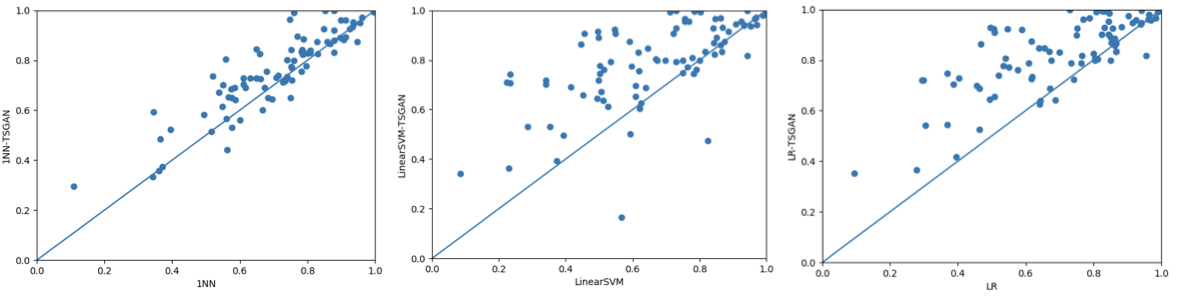
\includegraphics[scale=0.8]{figures/gan/acc.png}
\caption{分类比较结果}
\label{fig:gan-acc-knn}
\end{figure}

% \begin{figure}[H]
% \centering
% 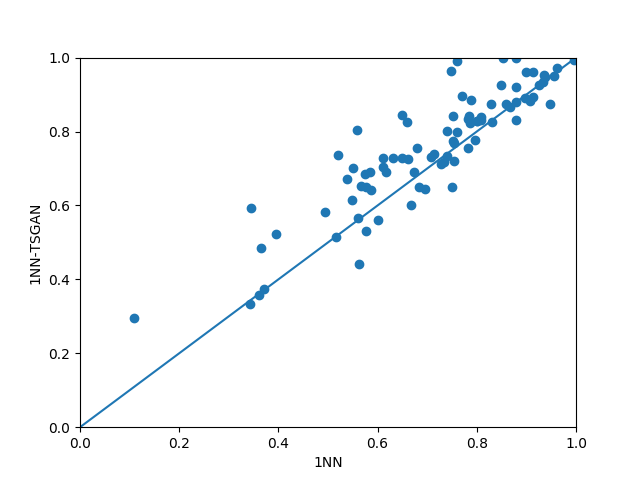
\includegraphics[scale=0.5]{figures/gan/0000_acc_knn.png}
% \caption{KNN 分类比较结果}
% \label{fig:gan-acc-knn}
% \end{figure}

% \begin{figure}[H]
% \centering
% 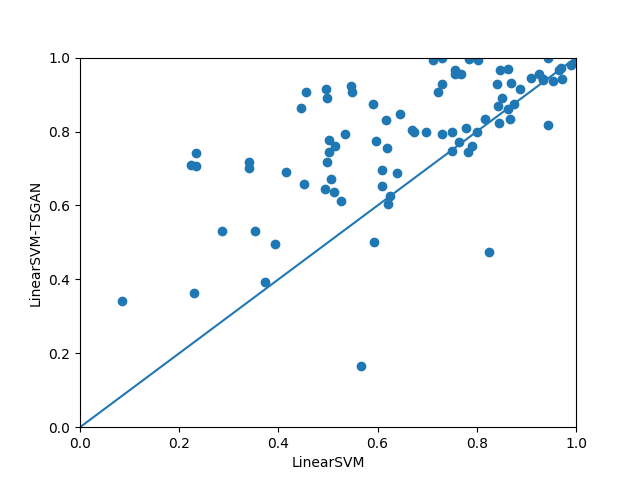
\includegraphics[scale=0.5]{figures/gan/0000_acc_lsvc.png}
% \caption{LinearSVM 分类比较结果}
% \label{fig:gan-acc-lsvc}
% \end{figure}

% \begin{figure}[H]
% \centering
% 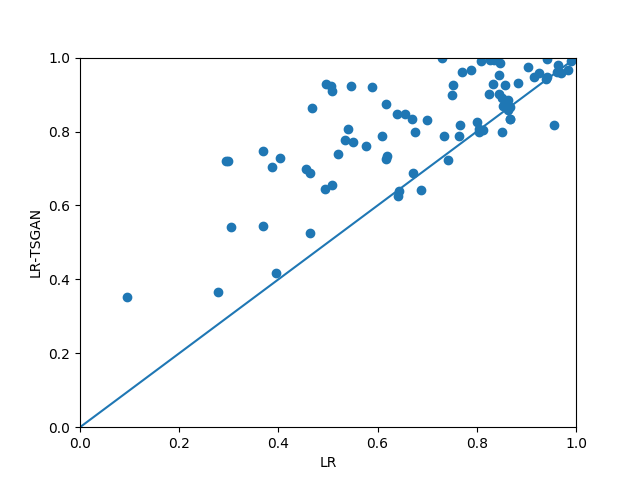
\includegraphics[scale=0.5]{figures/gan/0000_acc_lr.png}
% \caption{LR 分类比较结果}
% \label{fig:gan-acc-lr}
% \end{figure}

\section{小结}

%作为全文扩展,本章针对普遍存在的时间序列数据结合卷积神经网络和生成式对抗网络提出时间序列生成式对抗网络 (TSGAN)
本章结合卷积神经网络和生成式对抗网络提出无监督式时间序列通用特征学习框架TSGAN并基于此设计半监督式时间序列分类框架。

本文首先针对工业领域的重要数据资源——时间序列,进行广泛而深入的调研。然后针对时间序列高维、高噪、时变的特性以及由此导致的分析难和标记难的问题,结合卷积神经网络和生成式对抗网络提出了无监督式时间序列通用特征学习框架TSGAN并基于最大的时间序列分类数据集进行实验,数据集包含85个时间序列数据集,有基于加速计采集的运动时间序列、基于形状的时间序列数、基于传感器采集的频谱时间序列、医疗时间序列和工业系统时间序列。一方面,TSGAN的生成器可有效学习时间序列数据集的分布并生成逼真的多样化的时间序列,可作为模拟器使用;另一方面,TSGAN的判别器作为特征转换器与K近邻、支持向量机和逻辑斯蒂回归分类器结合形成半监督式时间序列分类框架并且取得优秀的分类效果,充分证明TSGAN学习了时间序列数据的关键特征。

本章工作,一方面首次基于生成式对抗网络提出无监督式时间序列特征学习的通用解决方案,丰富了GAN在时间序列领域的应用;另一方面,基于大量数据集验证模型效果,充分证明TSGAN对时间序列数据的普遍适用性以及其所学特征的有效性,为无监督式时间序列特征学习提供了新思路;再一方面,首次将生成式对抗网络成功应用于时间序列分类任务并取得优秀效果,为时间序列分类以及其他基于时间序列的机器学习任务提供新思路。

% # data parameter
% self.X = X
% self.img_h = img_h
% self.img_w = img_w
% self.c_dim = c_dim
% self.z_dim = int(X.shape[1] * 0.7)
% #self.z_dim = 100
% # model parameter
% self.gf_dim = 64  # dimension of G filters in first conv layer
% self.df_dim = 64  # dimension of D filters in first conv layer
% # training parameter
% self.nbatch = min(20, len(self.X))
% self.g_learning_rate = 0.0002
% self.d_learning_rate = 0.0002
% self.g_beta1 = 0.5
% self.d_beta2 = 0.5
% self.nepoch = 200
% self.k = 1
% # log parameter
% self.data_name = data_name
% self.file_name = out_fname
% self.model_name = "{}_{}".format(self.file_name, self.data_name)
% self.freq_print = 1
% self.freq_plot = 20
% self.freq_log = 20
% self.nsample = 10000
% self.dir_root = '/home/hfl/dataset/output/gan_timeseries_tf/{}'.format(self.file_name)
% self.dir_root_dataset = '{}/{}'.format(self.dir_root, self.data_name)
% self.dir_logs = os.path.join(self.dir_root_dataset, 'logs')
% self.dir_samples = os.path.join(self.dir_root_dataset, 'samples')
% self.dir_checkpoint = os.path.join(self.dir_root_dataset, 'checkpoint')

% # construct log file
% if state == 'train':
%     if os.path.exists(self.dir_root_dataset):
%         shutil.rmtree(self.dir_root_dataset)
%     os.makedirs(self.dir_root_dataset)
%     os.makedirs(self.dir_logs)
%     os.makedirs(self.dir_samples)
%     os.makedirs(self.dir_checkpoint)
